\documentclass[12pt]{report}

\usepackage[a4paper,
			inner = 35mm,
			outer = 25mm,
			top = 25mm,
			bottom = 25mm]{geometry}
\usepackage{lmodern}
\usepackage[magyar]{babel}
\usepackage[utf8]{inputenc}
\usepackage[T1]{fontenc}
\usepackage[hidelinks]{hyperref}
\usepackage{graphicx}
\usepackage{amssymb}
\usepackage{setspace}
\usepackage[nottoc,numbib]{tocbibind}
\usepackage{amsthm}
\usepackage{minted}
\usepackage{mdframed}
\usepackage{etoolbox}
\usepackage{xcolor}



% \setcounter{secnumdepth}{3}
\onehalfspacing

\newtheorem{mydef}{Definició}
\newtheorem{mytetel}{Tétel}
\newtheorem{mylemma}{Lemma}

\BeforeBeginEnvironment{minted}{\begin{mdframed}[backgroundcolor=bg, hidealllines=true]}
\AfterEndEnvironment{minted}{\end{mdframed}}

\newcommand{\cmd}[1]{\colorbox{gray!10}{\strut #1}}

\definecolor{bg}{rgb}{0.95,0.95,0.95}
\newminted[mintedJson]{js}{breaklines, breaksymbolleft=\quad}
\newminted[mintedBash]{bash}{breaklines, breaksymbolleft=\quad}



\begin{document}

\begin{titlepage}
	\begin{center}
		\vspace*{1cm}
		
		\textbf{\LARGE 
			Forgalom igény tudatos hálózat tervezés minimális torlódással és úthosszal
		}
	
	
		\vspace{0.5cm}
	
		\textbf{\normalsize Tudáskezelő rendszerek III. labor összefoglaló}
		
		\vfill
		
		\Large Szecsődi Imre
		
		\vspace{2.8cm}
		
		\the\year
		
	\end{center}
\end{titlepage}

\tableofcontents
	
\chapter{Bevezetés}


\section{Labor célja}

A labor célja a korábban már bemutatott cikkben\cite{avin_demand-aware_nodate} szereplő hálózat építése.
Az eredeti cikkben a fák építésére az Egofa algoritmus volt használva. 
A labor keretén belül azt a felvetést vizsgáltam meg, hogy lehet-e jobb algoritmust találni fa építésre, mint az Egofa.  
Az új módszerek hasonlóan az eredetihez véletlenszerűen generált gráfokra voltak tesztelve.
Az így kapott eredmények a különböző algoritmusokból az eredeti eredménnyel voltak összehasonlítva.

\section{Laborban megvalósított munka}

A labor ideje alatt a már elkészült keretrendszer adta az alapot, ami segítségével tesztelhető a szerzők által felvázolt és három saját fejlesztésű algoritmus.
A keretrendszer Python \cite{noauthor_python_nodate} nyelven íródott.
A véletlen gráfok generálására a NetworkX külső csomag volt használva\cite{noauthor_networkx_nodate}.
Az adatok elemzése RapidMiner-ben történt\cite{noauthor_lightning_nodate}.

\chapter{Modell}

\section{Az új algoritmusok}

\subsection{Egobalance}

Az első algoritmus majdnem teljes mértékben megegyezik az eredetivel.
A cikk szerzői az Egofa algoritmus vázlatos összefoglalásában használtak egy csere lépést.
A csere lépés lényege, hogy mikor megépítettük a fát egy magas csúcsra akkor a fában minden szomszédja megjelenik.
A szomszédok között megtalálhatók a magas-magas fokszámú kapcsolatok, amiket ki kell cserélni a segítő csúcsokra.
Három esetet különböztetünk meg itt, attól függően hol helyezkedik el a segítő csúcs a fában.
Első eset, mikor a segítő csúcs nem szerepel a fában, ilyenkor a magas csúcsot ki kell cserélni a segítőre. Ebben az esetben nem kell semmi kiegészítő lépést csinálni, mivel a gyerekeket átveszi a segítő.
A következő két eset, mikor a segítő pont is része a fának, attól függően mennyire közel vannak az érintett csúcsok a fa gyökeréhez más-más gyerek csúcsokat kell újra elhelyezni.
Mikor a segítő csomópont közelebb van a gyökérhez akkor töröljük a magas pontot a fából, ha voltak gyerekei a törölt pontnak, akkor azoknak új szülő csúcsot kell találni.
Ellenkező esetben, mikor magas pont helyezkedik el közelebb a forráshoz, akkor a segítő csúcs átveszi a helyét és gyerekeit, majd a segítő leveleinek kell új szülő csúcsot találni. 
Ezt úgy oldja meg az eredeti algoritmus, hogy a nehezebb levél csúcs lesz az új szülő és a könnyebb csomópontnak ő lesz a szülője.

Egy lehetséges eset ilyenkor, hogy az új szülő csúcsnak már ki van töltve mindkét levele, ekkor a szülő könnyebb levele fog egyel lejjebb szintre kerülni.
Ezt a folyamatot addig ismételjük, még minden levél nem kerül egy megfelelő helyre.
Az Egobalance logaritmus a függő pontok újra elhelyezését az Egofára bízza, azaz újra elosztásra kerülnek.
Ezzel elméletben mindig arra törekszik az algoritmus, hogy optimális legyen torlódásra nézve az új fa.
Lényegi különbség úthossznál jelentkezik az eredetivel szemben.

\subsection{Huffman fa}

A eddigi két algoritmus az Egofát\cite{avin_demand-aware_nodate} használta, ami optimális torlódásra nézve, de mivel a hálózat nem csak torlódás szempontjából van vizsgálva, ezért meg kell vizsgálni a másik aspektust is, az optimális úthosszt.
A Huffman kódolásnál\cite{huf52} használt fa tulajdonsága, hogy átlagosan rövidek legyenek az utak attól függően milyen gyakori egy elem.
A cl-Dan probléma is ezt a tényezőt használja, ezért kitűnően lehet használni ezt a fát a hálózat alapjának.
Egyetlen probléma a Huffman fával az, hogy a belső csomópontok nem tartalmaznak számunkra hasznos információt.
Ezért szükséges egy kiegészítő lépés, ami segítségével belső pontok is ki lesznek töltve, azaz esetünkben csomópontokat fognak reprezentálni, amik maguk is végpontok mint a levelek.

Az algoritmus első része teljesen megegyezik a Huffman kódolással.
Rendezzük sorba növekedően a pontokat, és kettesével vonjuk össze őket, még nem kapunk egy teljes fát.
Mint az Egofáknál, úgy a Huffman fánál is a legfelső szinten \(n\) darab csúcsot tudunk a forrás pontra kapcsolni.
Az összes többi alacsonyabb pont pedig marad bináris.

A belső pontok kitöltésére a következő algoritmust végezzük el az összes gyökérre kapcsolódó ágon:
\begin{enumerate}
	\item Gyűjtsük össze a levelet az ágon, mivel a levelek tartalmaznak hasznos pontokat számunkra
	\item Az csúcsokból kezdjünk el egy sorfolytonos fát építeni, ahol a valószínűségek csökkenő sorrendben vannak elhelyezve
\end{enumerate}
 
Felmerülhet a kérdés, hogy miért nem a legnehezebb levél jön fel mindig?
Ez azért van, mert a Huffman kódolásnál megtörténik az az eset, hogy két csomópont összesített értéke megegyezik egy harmadikkal.
Ez olyan fát eredményez, ahol bal oldalon egy nehéz csúcs és jobb oldalon egy fában két könnyű csomópont szerepel.
A naiv megoldás esetén ez azt eredményezi, hogy az egy nehéz pont lesz a belső csúcs és az ág ahonnan jött megüresedik.
A pont levelei nem fognak ágat változtatni, annak ellenére, hogy megüresedett az egyik feljebb, ezért hosszú egyenes utak jöhetnek létre.
Ennek kiküszöbölésére van a sorfolytonos algoritmus, ahol garantálni lehet, hogy fa egyik belső pontja sem marad kitöltetlen.

\subsection{Sorfolytonos fa}

Mint láthattuk korábban a Huffman fánál, a levelek felfelé mozgatását sorfolytonosan valósítottuk meg. A sorfolyonos fa is hasonló elvet követ.
Lényegi különbség a kettő fa között, hogy a Huffman kódolási algoritmust kihagyjuk, és egyenest sorfolytonosan rakjuk fel csúcsokat a fa építésekor.
Ezzel mindig a legkisebb fákat kapjuk, de ez a torlódást egyáltalán nem veszi figyelembe.

\chapter{Megvalósítás}


\section{Adatszerkezetek}

A modell alapját pár egyszerű alaptípus adja. Ezek rendre a következők:
\begin{itemize}
	\item \textbf{Vertex} - az általános gráf csúcs
	\item \textbf{Node} - az \textit{Egófák} készítésekor használt csúcs, ami tartalmazza a valószínűségét annak, hogy a forrás csomópont mekkora valószínűséggel fog kommunikálni a másik \textit{Node} csúccsal
	\item \textbf{HuffmanDanNode} - a Huffman fa csomópontjait reprezentáló osztály, minden tulajdonsága megvan mint a Node-nak, csak még kiegészül egy útvonallal, amit a Huffman fa építése után lesz meghatározva
	\item \textbf{Edge} - az gráf pontjait összekötő él reprezentációja, ami \textit{Vertexet} vár paraméterként, és tartalmazza a kommunikációs valószínűséget, hasonlóan mint a \textit{Node}
	\item \textbf{Tree} - ami adja az alapját majd a útvonal tervezési sémának. A fának két fajtája van megvalósítva:
	\begin{itemize}
		\item \textbf{EgoTree} - a $\Delta$ fokú Egofa, ahol a gyökérnek legfeljebb $\Delta$ levele lehet
		\item \textbf{HuffmanDanTree} - a $\Delta$ fokú Huffman fa, ahol a gyökérnek legfeljebb $\Delta$ levele lehet és a belső csúcsok állhatnak üresen
	\end{itemize}

	
\end{itemize}
	
\section{Modell}

A \textbf{Network} osztály megváltozott az előző megvalósításhoz képest.
Absztrakt osztályra lett átalakítva, a belőle leszármazó osztályok valósítják meg a különböző algoritmusokat.
A leszármaztatott osztályoknak egyetlen függvényt kell csak megvalósítani, ami a fa építései stratégiát tartalmazza.
Ennek segítségével nagyon egyszerűen lehet új algoritmust illeszteni a már meglévő rendszerhez.

A bemeneti konfiguráció kiegészült egy új gráf típussal, ami a csillag gráf.
Csillag gráfnak nevezzük azt a gráfot, ahol az összes pont egy ponthoz kapcsolódik.
A konfiguráció további egységesítésen esett át, minden véletlen gráf szerkezete megegyezik, ami a következő:

\begin{itemize}
	\item \cmd{graph} - Gráf típusa, lehetséges értékek:
	\begin{itemize}
		\item \cmd{barabasei-albert} - Barabási-Albert gráf
		\item \cmd{erdos-renyi} - Erdős-Rényi gráf
		\item \cmd{star} - Csillag gráf
	\end{itemize}
	
	\item \cmd{vertex\textunderscore num} - Csomópontok száma
	\item \cmd{dan} - A maximális fokszám a magas fokú csúcsokra
	\item \cmd{constant} - Konstans érték ami a gráf paraméterét adja, ezek rendre a következők:
	
	\begin{itemize}
		\item Barabási-Albert gráf esetén azt határozza meg, hogy az új csúcs mennyi már a gráfban szereplő csúcshoz kapcsolódjon
		\item Erdős-Rényi gráf esetén az él valószínűségének meghatározásra használjuk a következő képlet segítségével  \[p = constant \cdot \frac{1}{vertex\_num}\]
		\item Csillag gráf esetén pedig a csillagok számát adjuk meg
	\end{itemize}
\end{itemize}

\chapter{Teszt eredmények}

\section{Tesztelés menete}

A tesztelés során mindegyik véletlen gráfok volt használva, és minden algoritmus ugyanazon a bemeneti mátrixon dolgozott a egyértelmű összehasonlítás érdekében. 
A mérések a konstans alapján lettek kiértékelve, mivel az a fő érték, ami alapján változik a gráf ritkasága.
A skálázhatóság tesztelésére különböző számú csúcs volt használva, ezek rendre: 11, 15, 35, 50, 75, 100, 125, 150, 175 és 200.
A skálázhatósághoz még hozzátartozik a maximum fokszám, hogy mennyi gráf csúcs tud egyszerre kommunikálni, ezért az is meg van adva.
A valóságban van egy fizikai határ, hogy mennyi kliens tud csatlakozni egyszerre, ezért az értékek így lettek megválasztva, 10, 16, 24 és 48.
A konkrét számú pont mellett meg volt vizsgálva az is, hogy valóságban mekkora szorzóra van szükségünk, mivel a cikk ad egy felső becslést ami $\Delta=12\rho$, ezért a teszt során figyelve volt az ajánlott és szükséges fokszám.
Az ajánlott fokszám értékei a következők voltak $\Delta\in[1\rho, 2\rho, 4\rho, 6\rho, 8\rho, 10\rho, 12\rho]$.
Az így megadott paraméterek alapján 52800 teszt lett lefuttatva.


\section{Eredmények}

\subsection{Átlag Súlyozott úthossz}

A következő grafikonok ábrázolják az eredményeket úthosszra nézve. 
Megfigyelhető, hogy az összes véletlen gráfon hasonlóan teljesítenek az algoritmusok.
A mátrix kitöltöttségének függvényével megegyezően növekedett az úthossz értéke is.
Egy érdekes megfigyelés még továbbá a tény, hogy mikor kicsi volt a konstans, feltehetően ritka mátrixot eredményezve magasabb eredményeket kapunk.
Ahogy növeljük a konstanst és több érték kerül be a mátrixba, több lehetőségünk lesz olyan segítő csúcs kiválasztására amit még nem használtunk korábban, ezzel rövidítve az utakat.

\begin{figure}[H]
	\begin{center}
		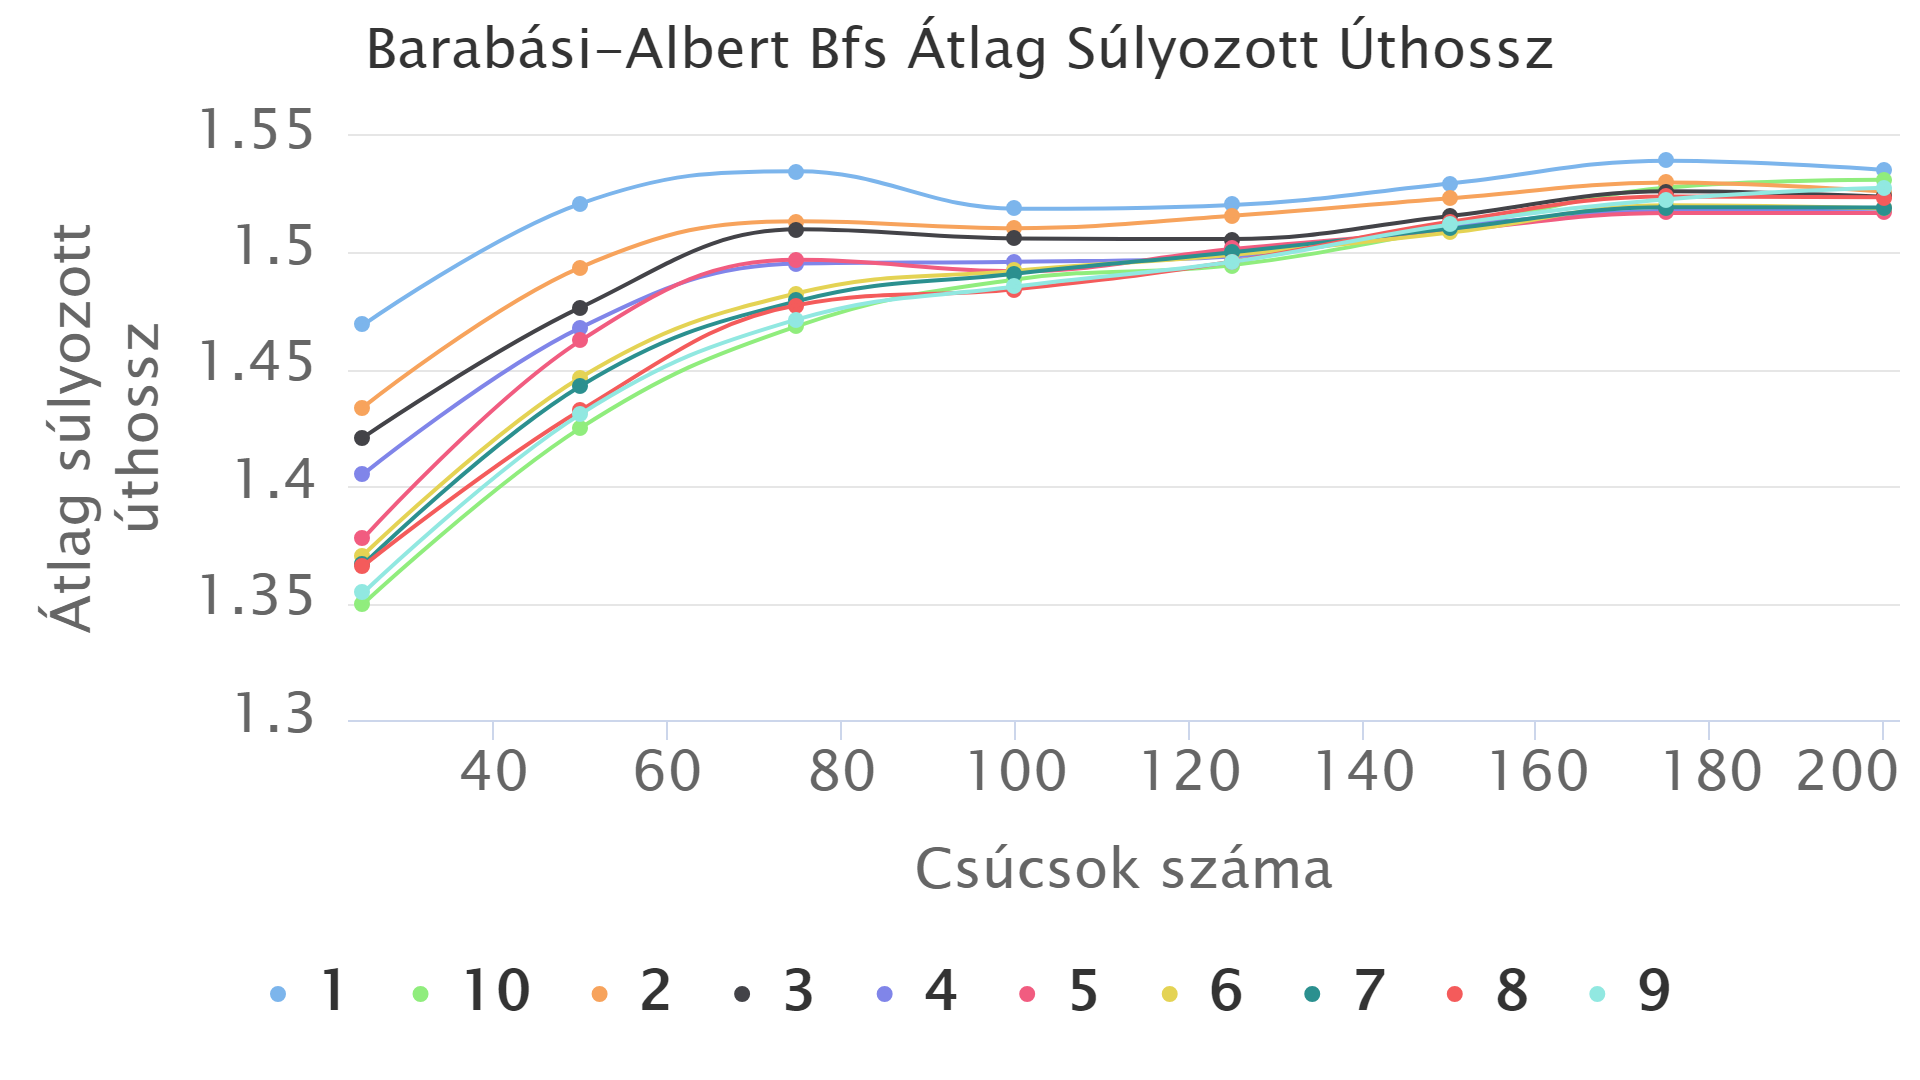
\includegraphics[width=0.49\linewidth]{pictures/barabasi_avg_len_bfs.png}
		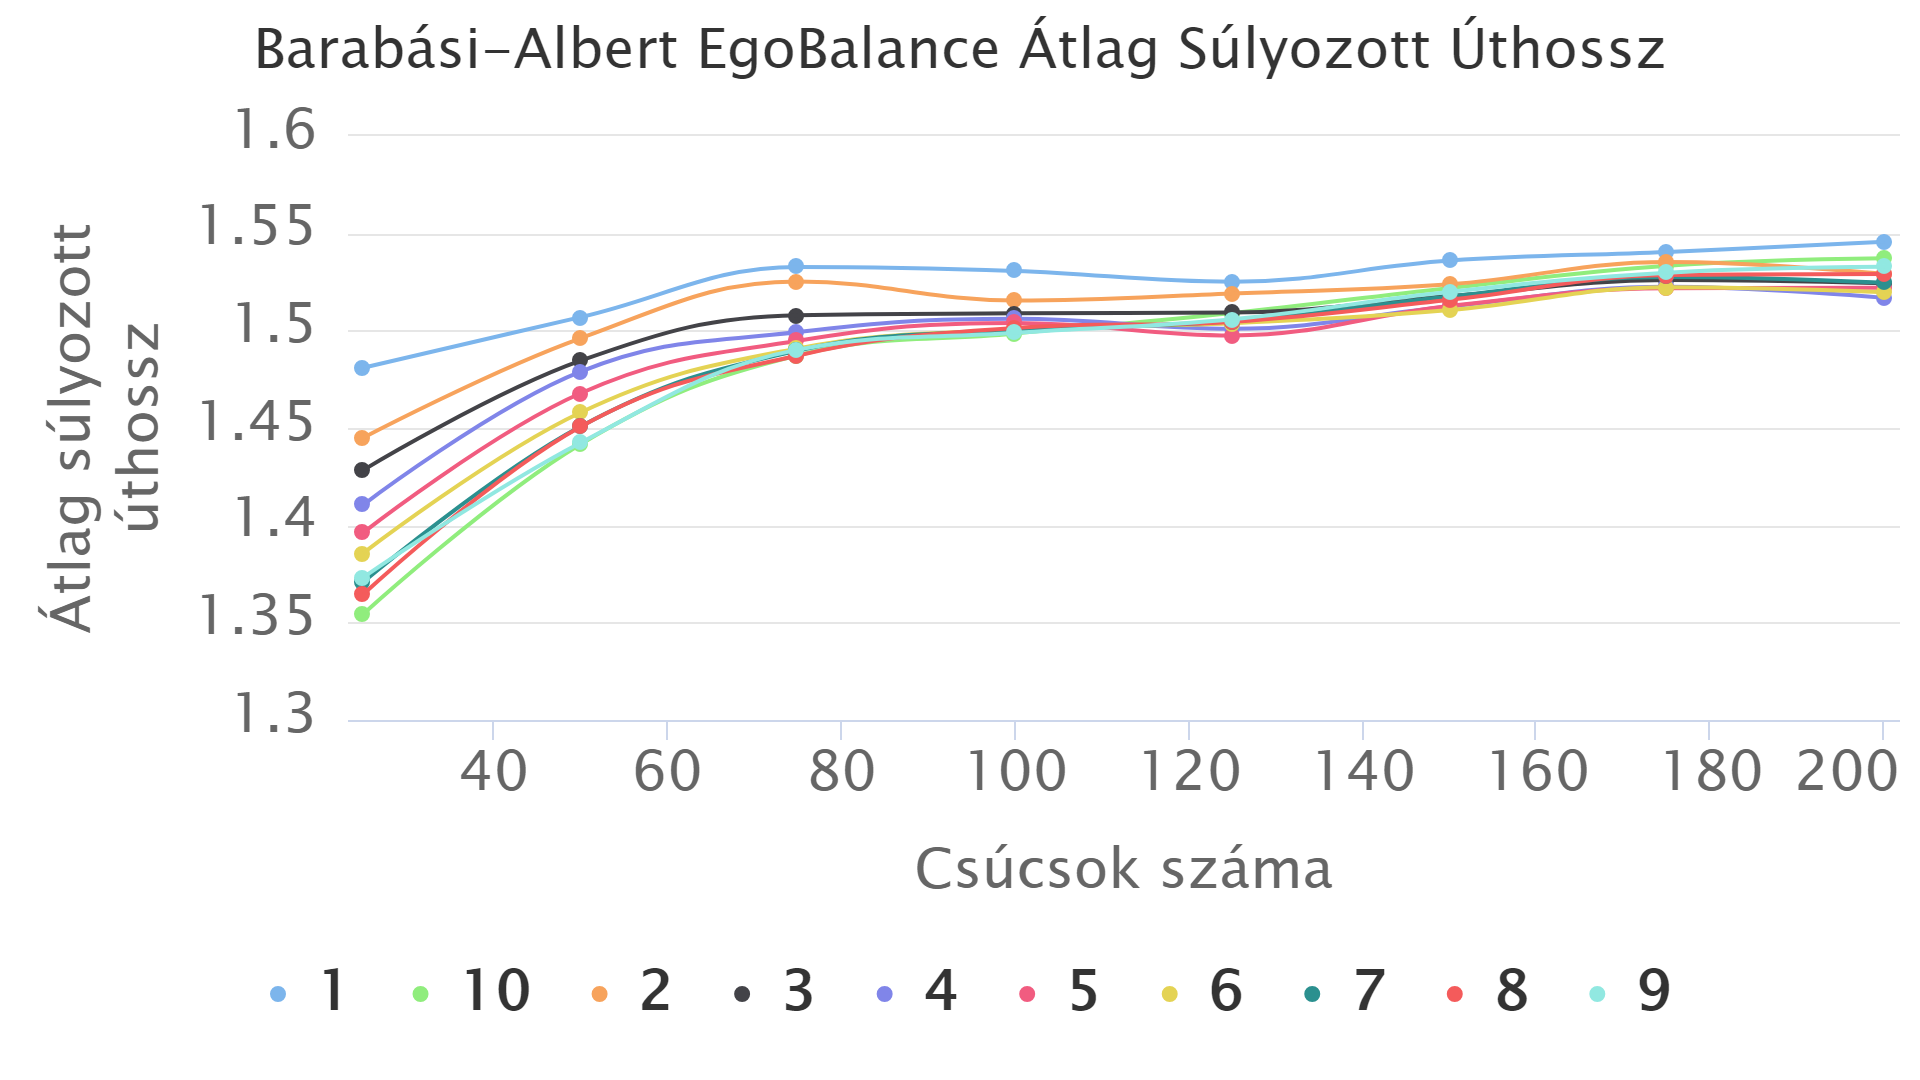
\includegraphics[width=0.49\linewidth]{pictures/barabasi_avg_len_egobalance.png}
		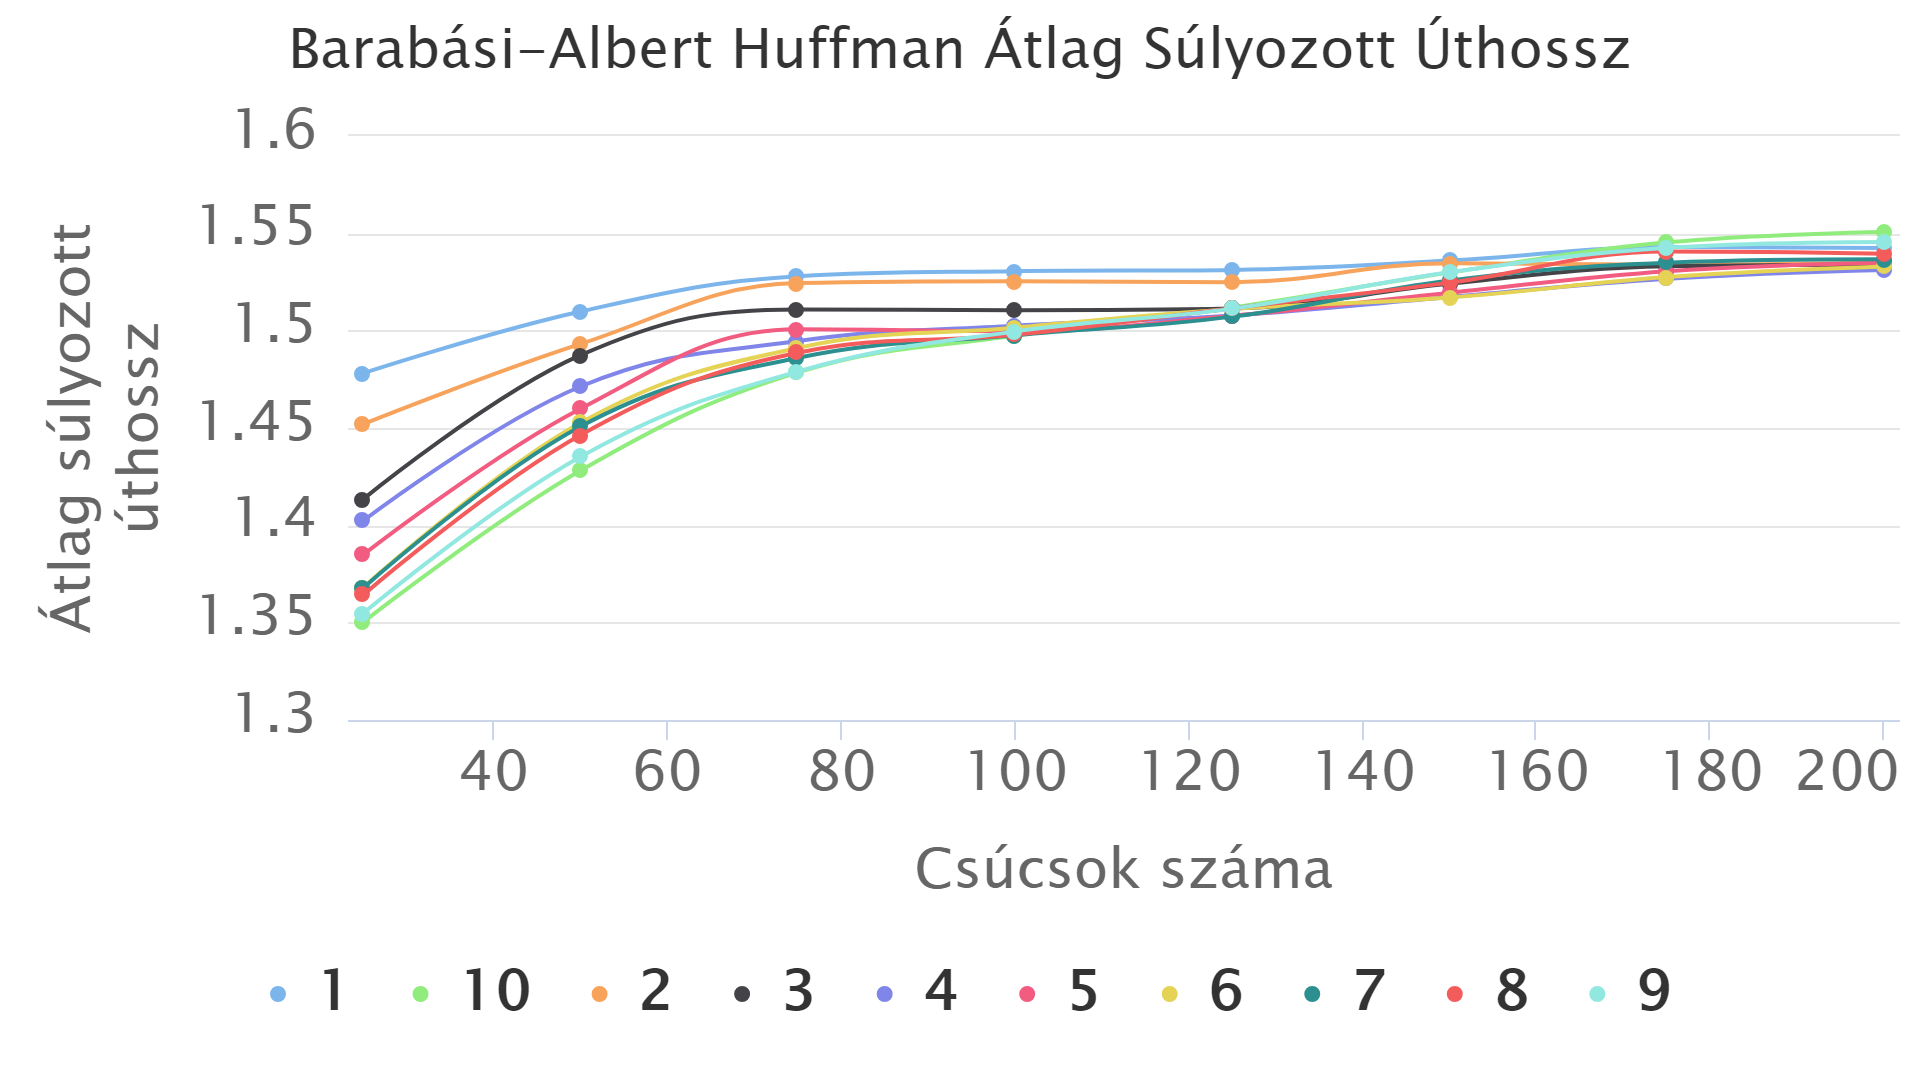
\includegraphics[width=0.49\linewidth]{pictures/barabasi_avg_len_huffman.png}
		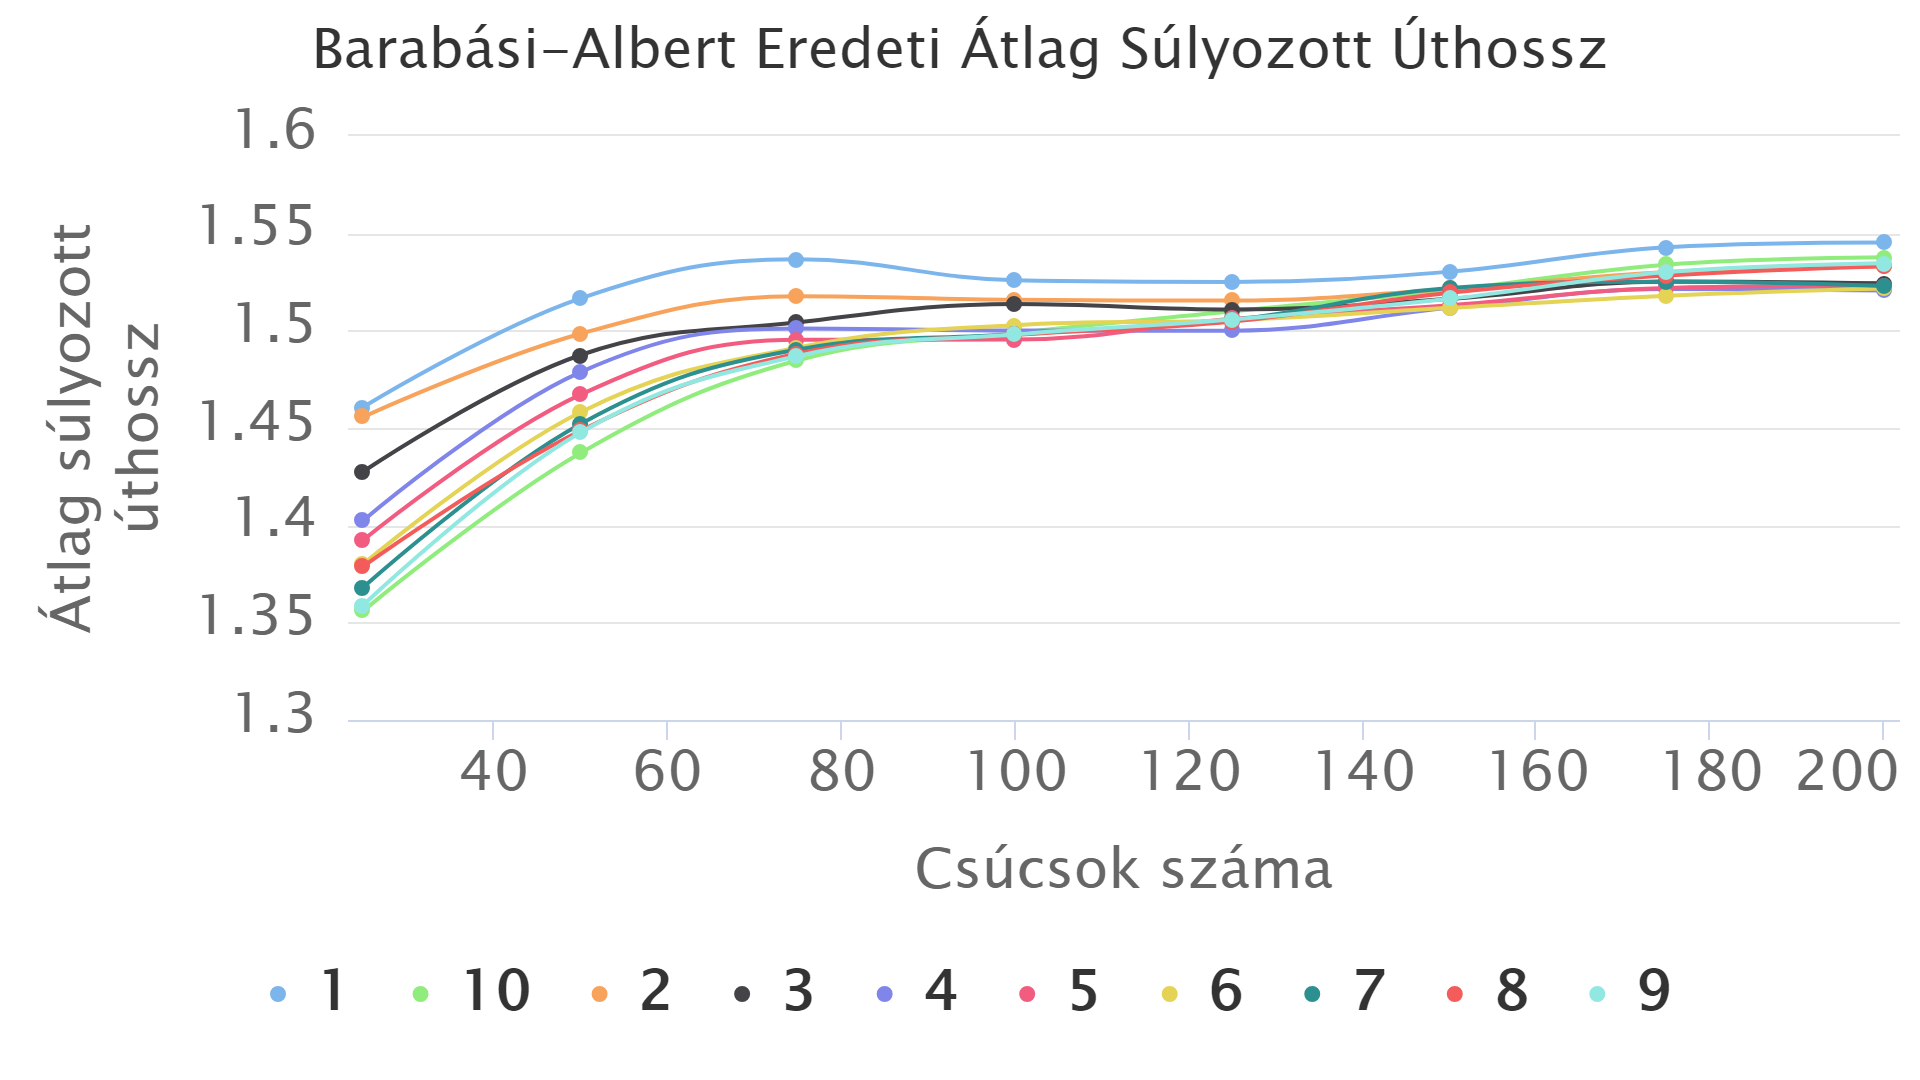
\includegraphics[width=0.49\linewidth]{pictures/barabasi_avg_len_original.png}
		\caption{Átlag súlyozott úthossz Barabási-Albert Gráf}
		\label{avg-len-barabsi}
	\end{center}
\end{figure}


\begin{figure}[H]
	\begin{center}
		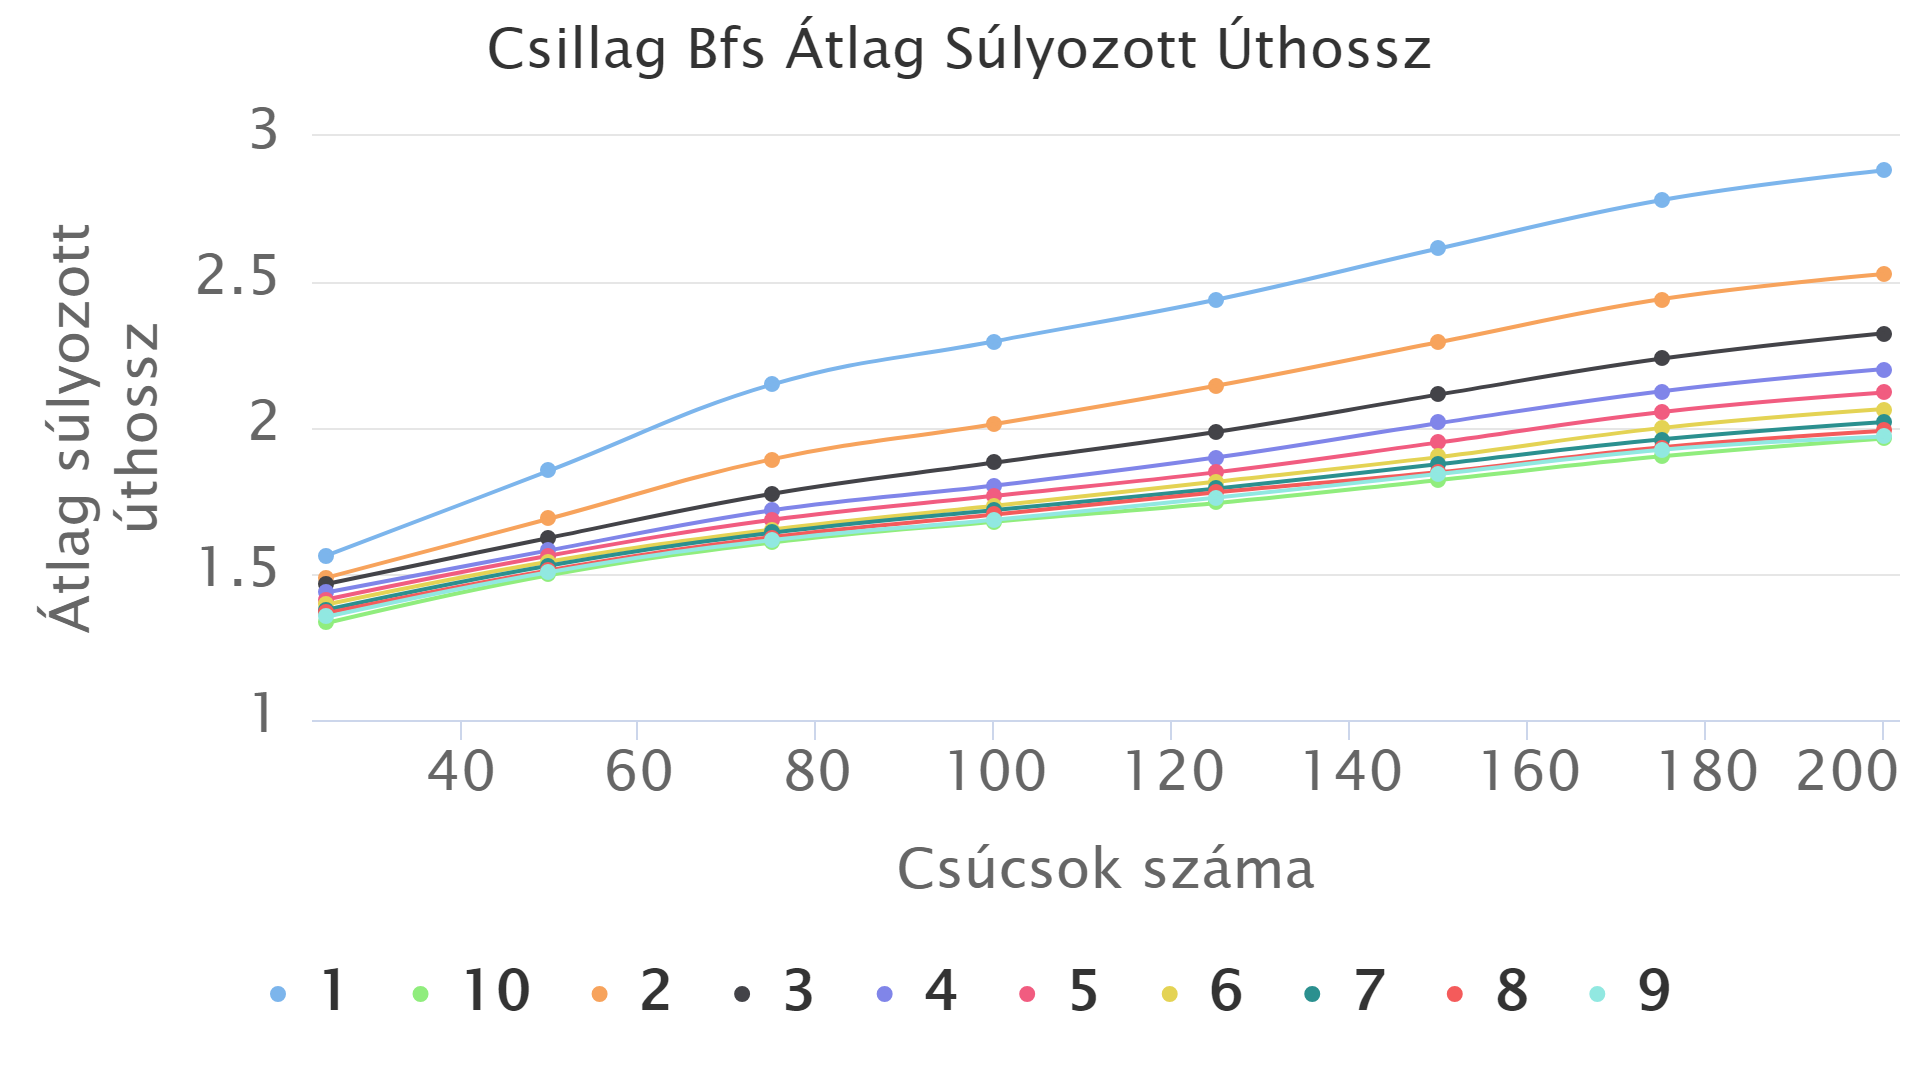
\includegraphics[width=0.49\linewidth]{pictures/star_avg_len_bfs.png}
		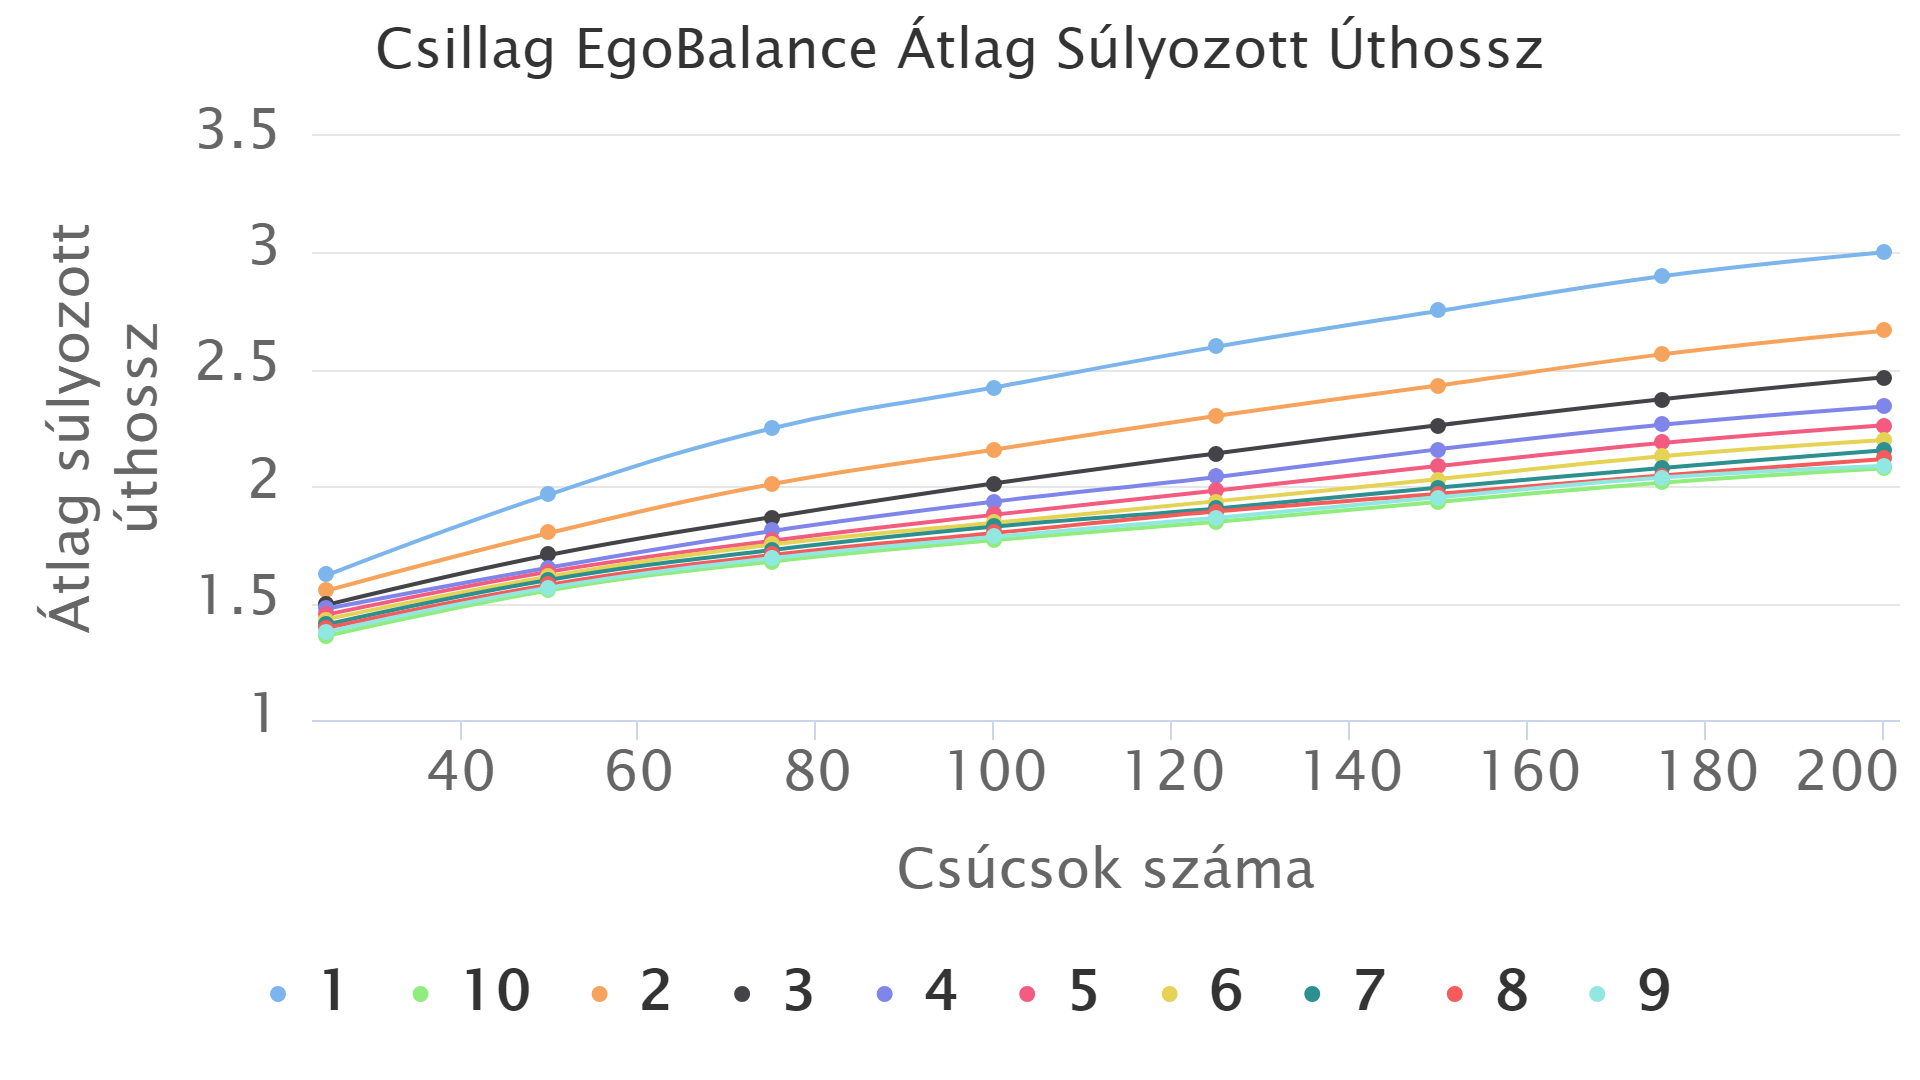
\includegraphics[width=0.49\linewidth]{pictures/star_avg_len_egobalance.png}
		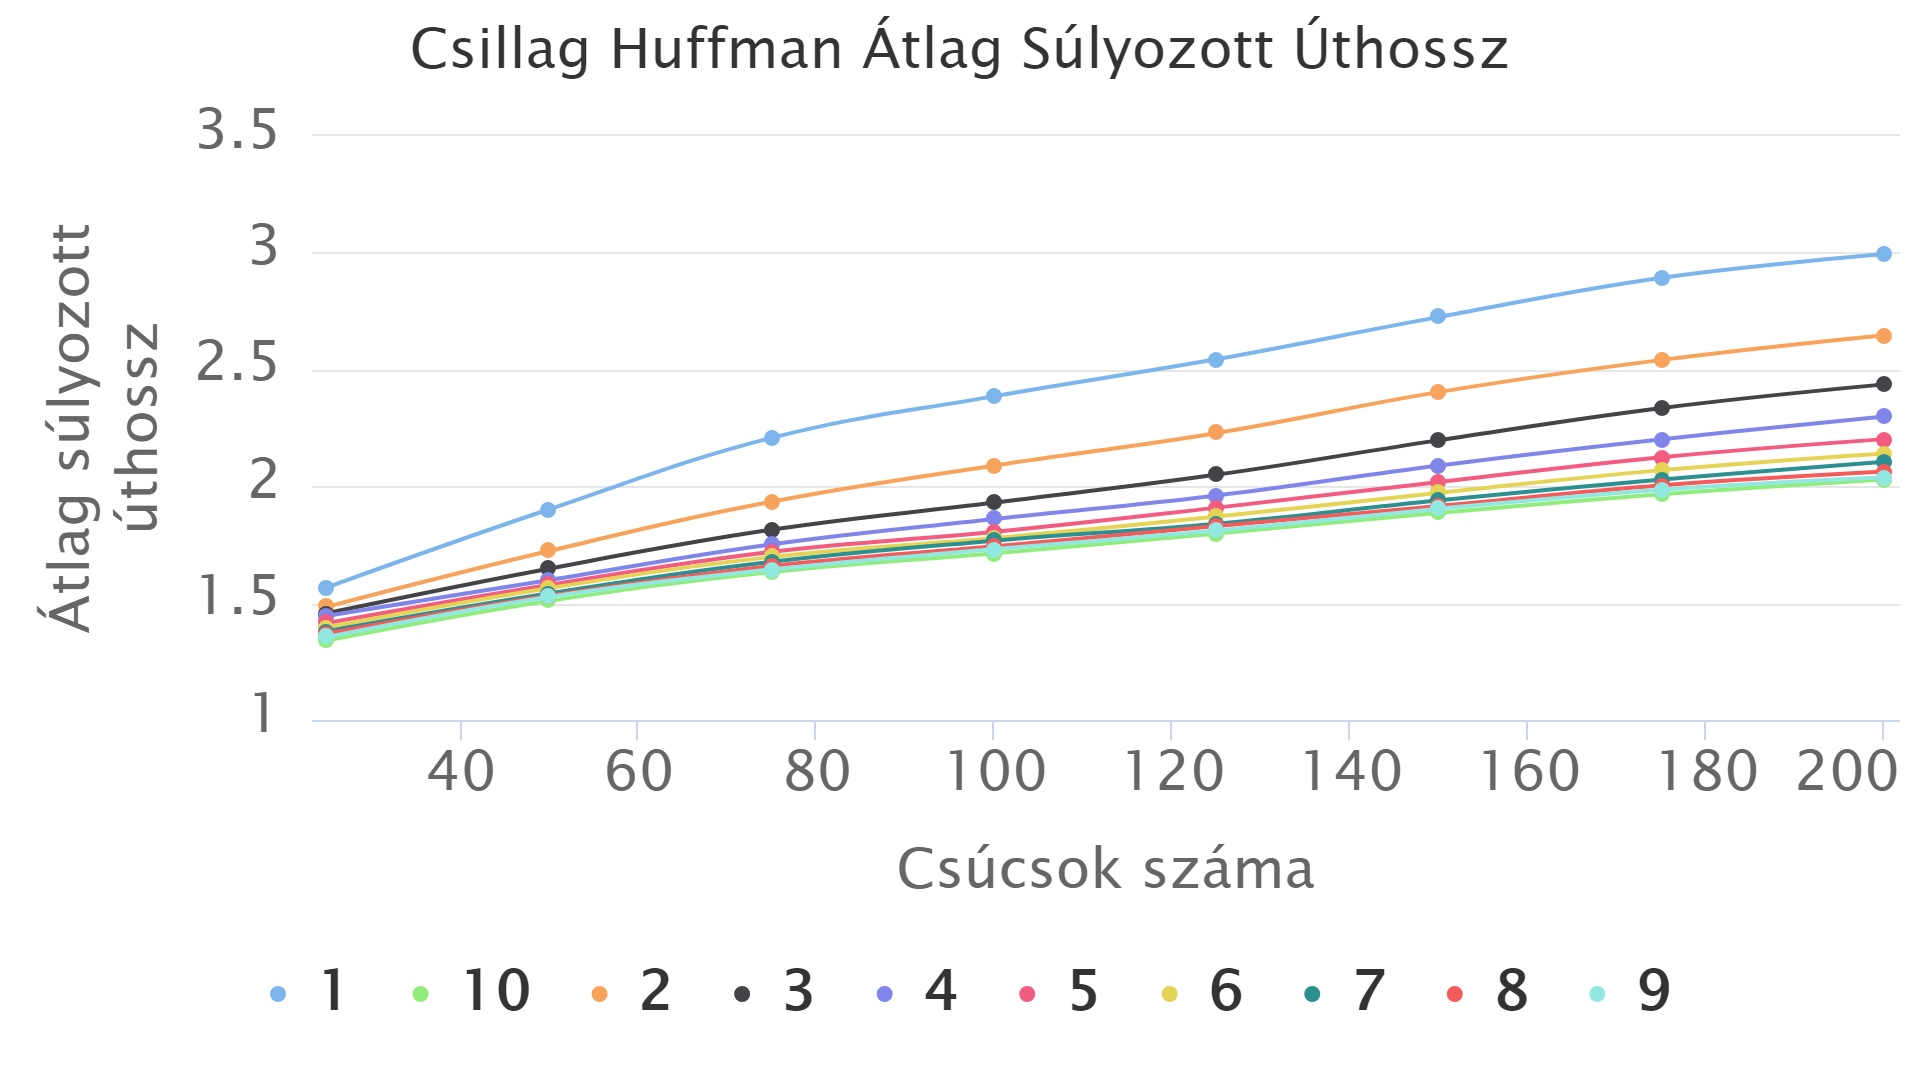
\includegraphics[width=0.49\linewidth]{pictures/star_avg_len_huffman.png}
		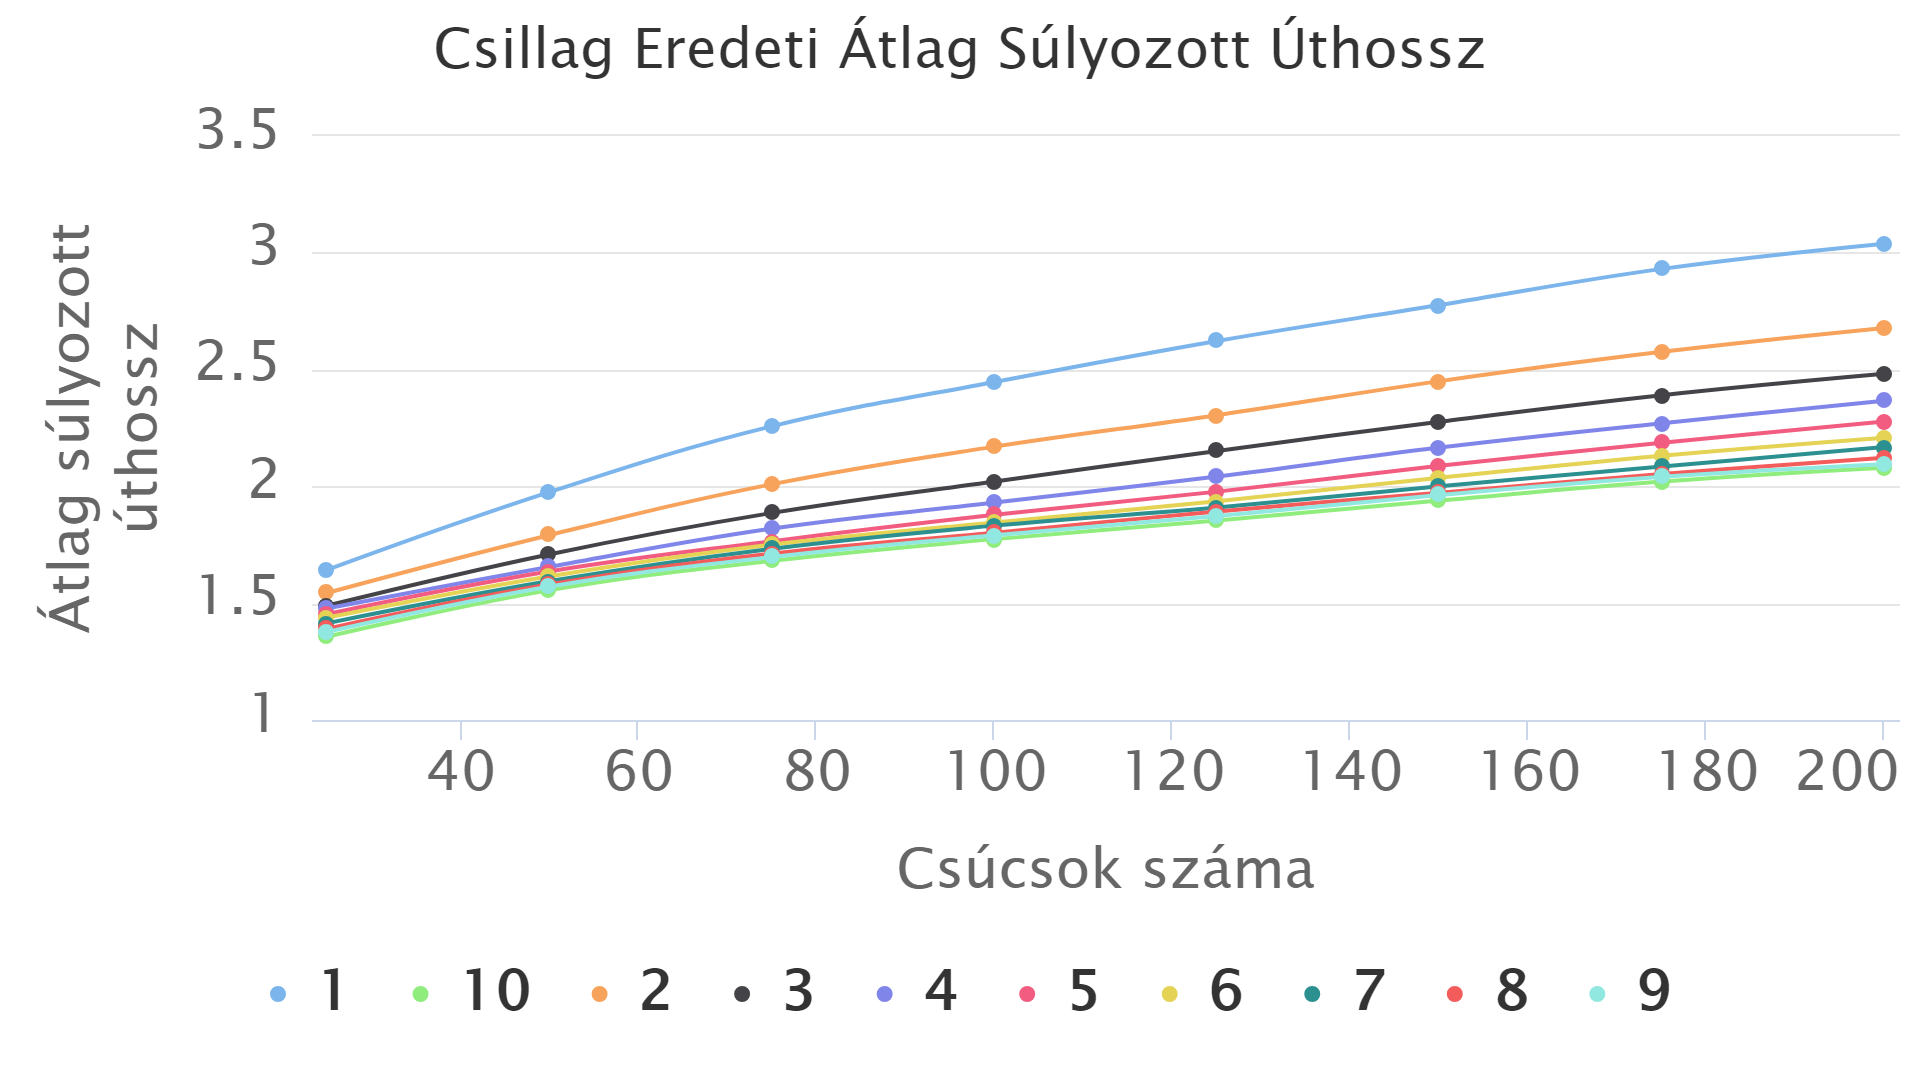
\includegraphics[width=0.49\linewidth]{pictures/star_avg_len_original.png}
		\caption{Átlag súlyozott úthossz Csillag gráf}
		\label{avg-len-star}
	\end{center}
\end{figure}

\begin{figure}[H]
	\begin{center}
		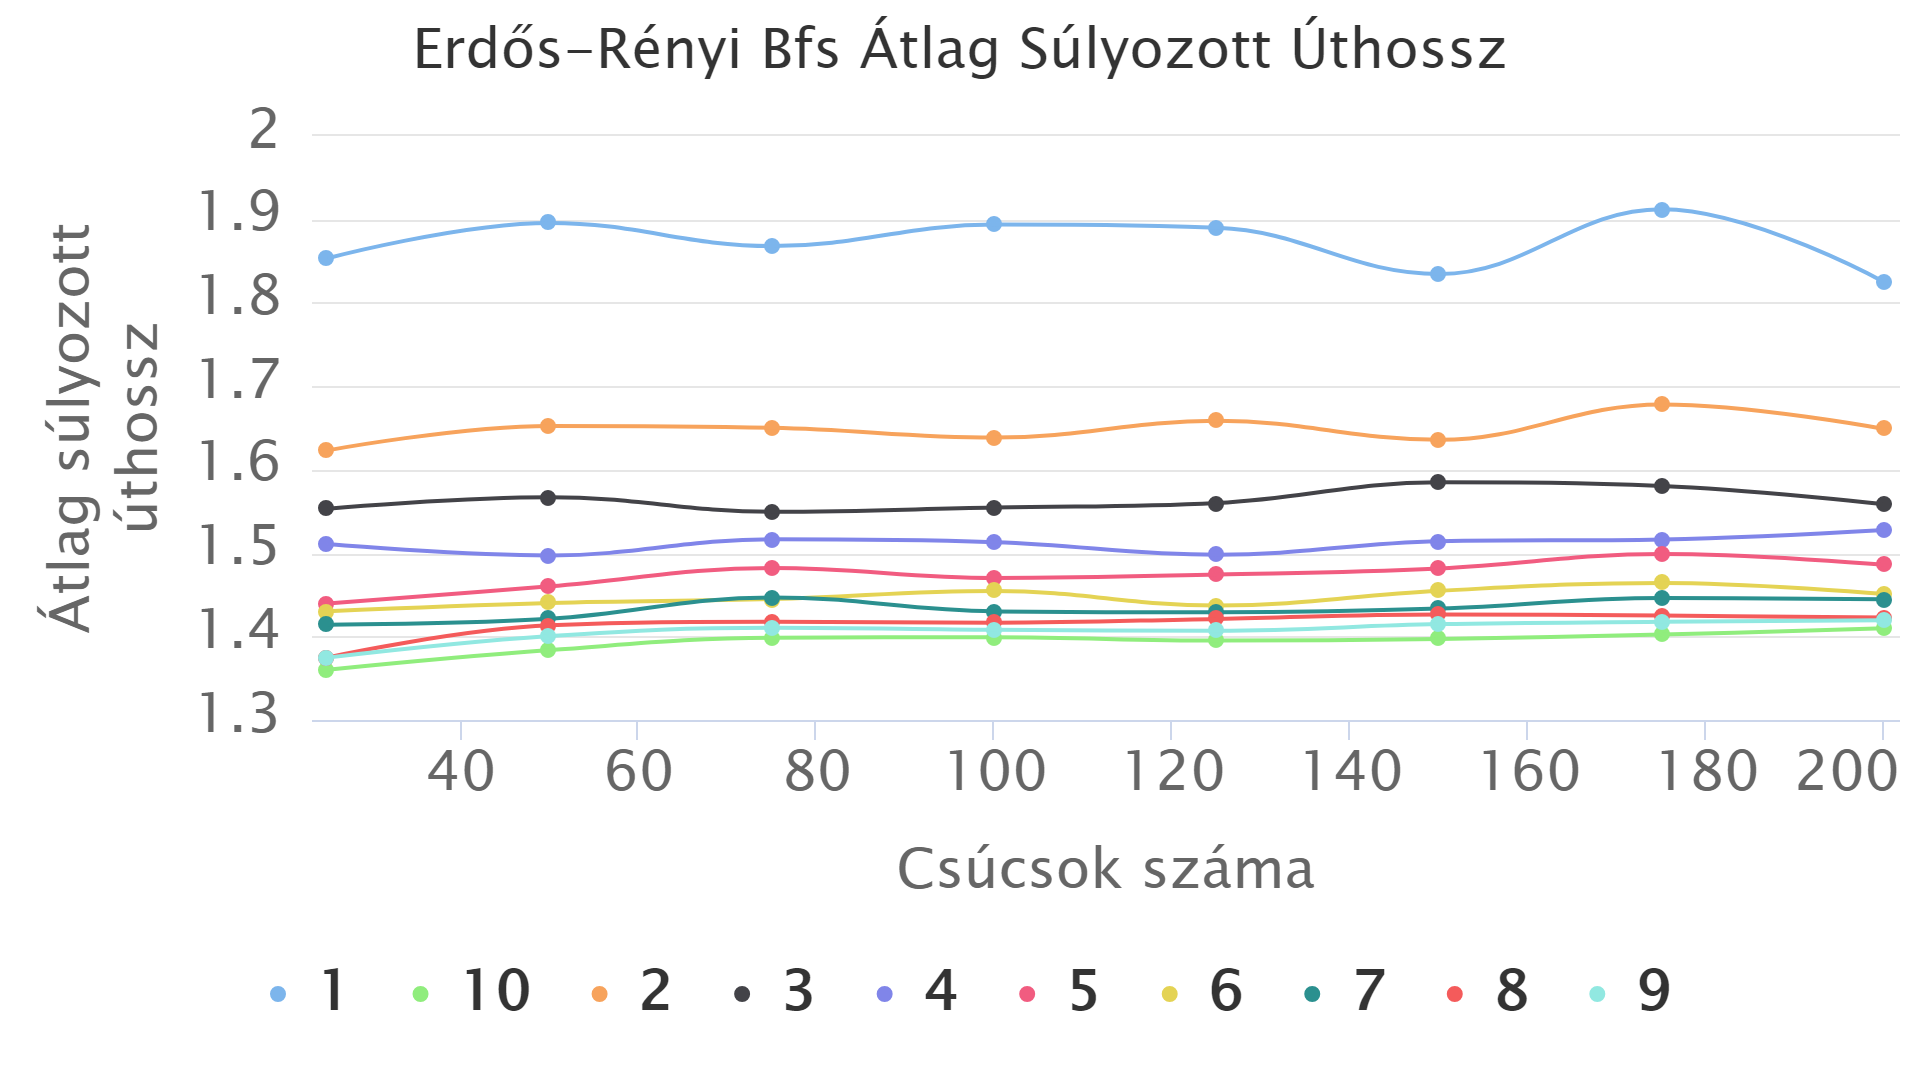
\includegraphics[width=0.49\linewidth]{pictures/erdos_avg_len_bfs.png}
		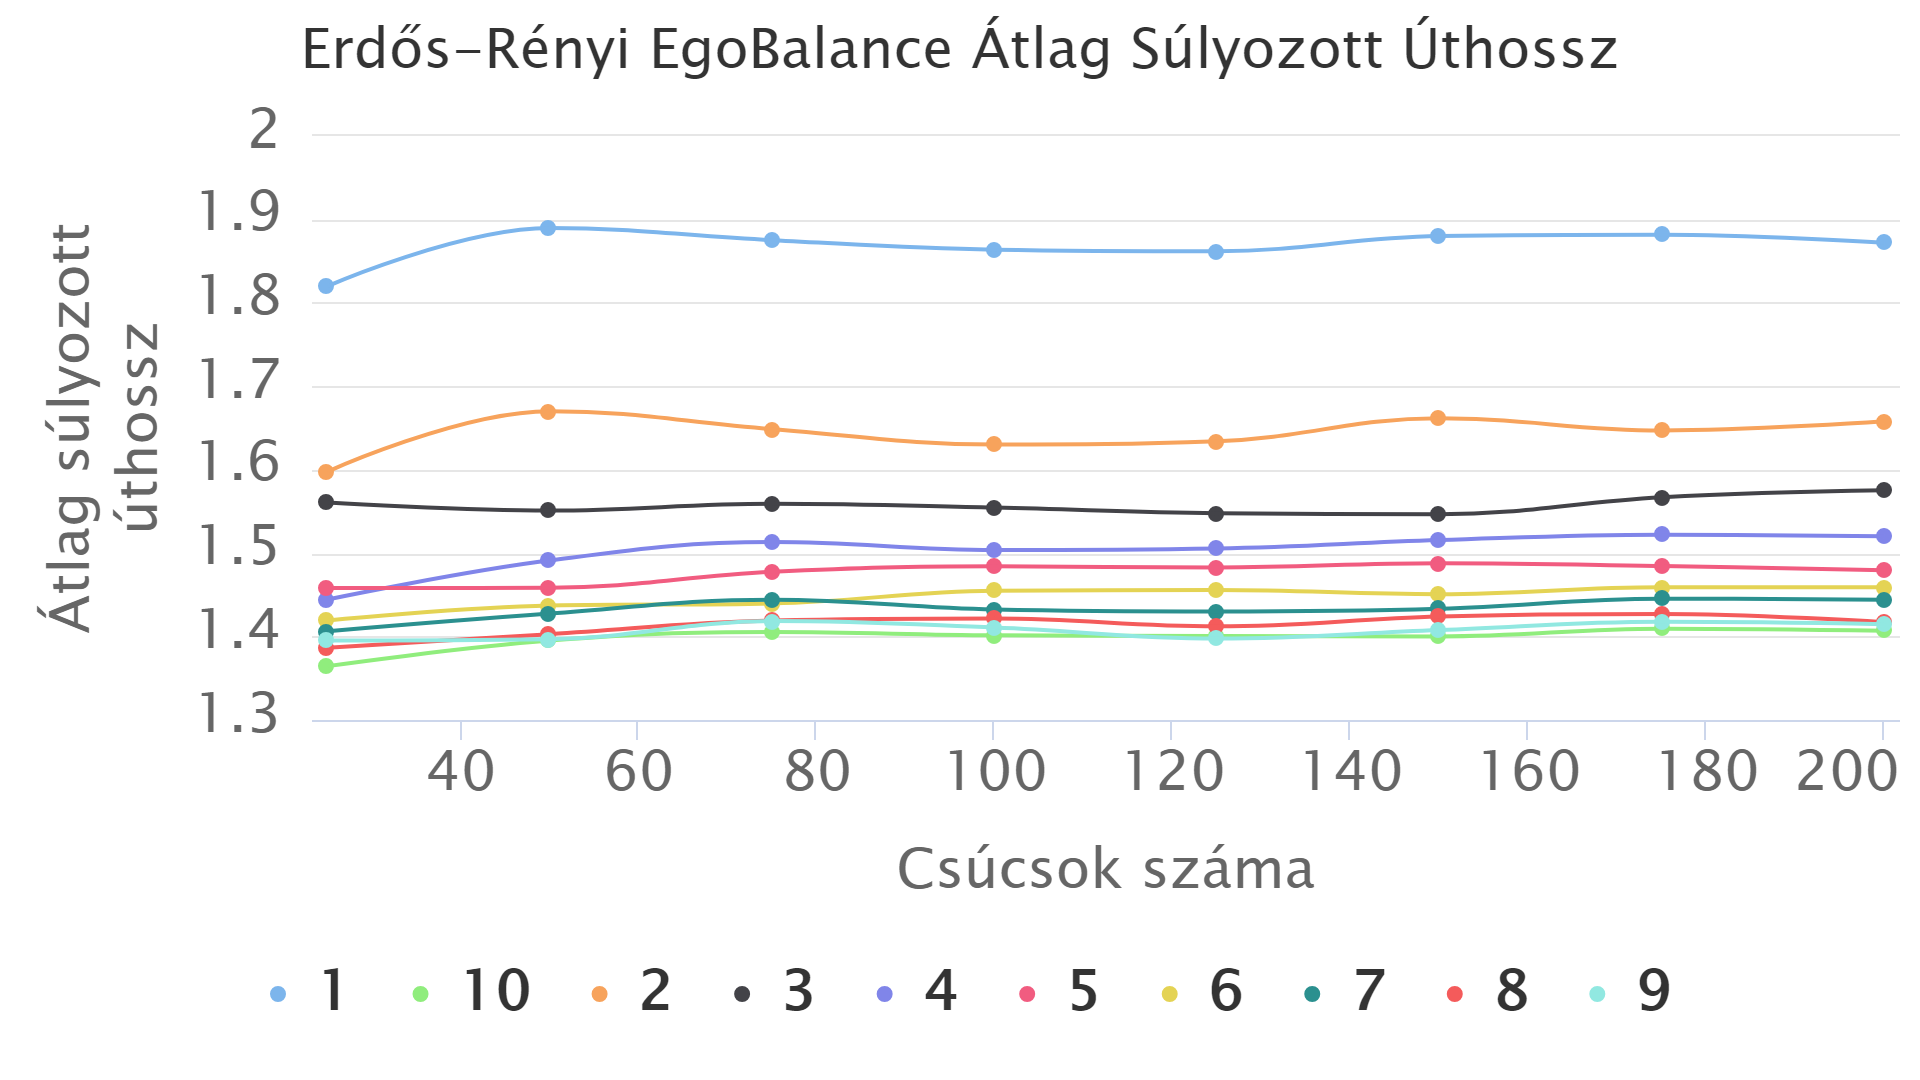
\includegraphics[width=0.49\linewidth]{pictures/erdos_avg_len_egobalance.png}
		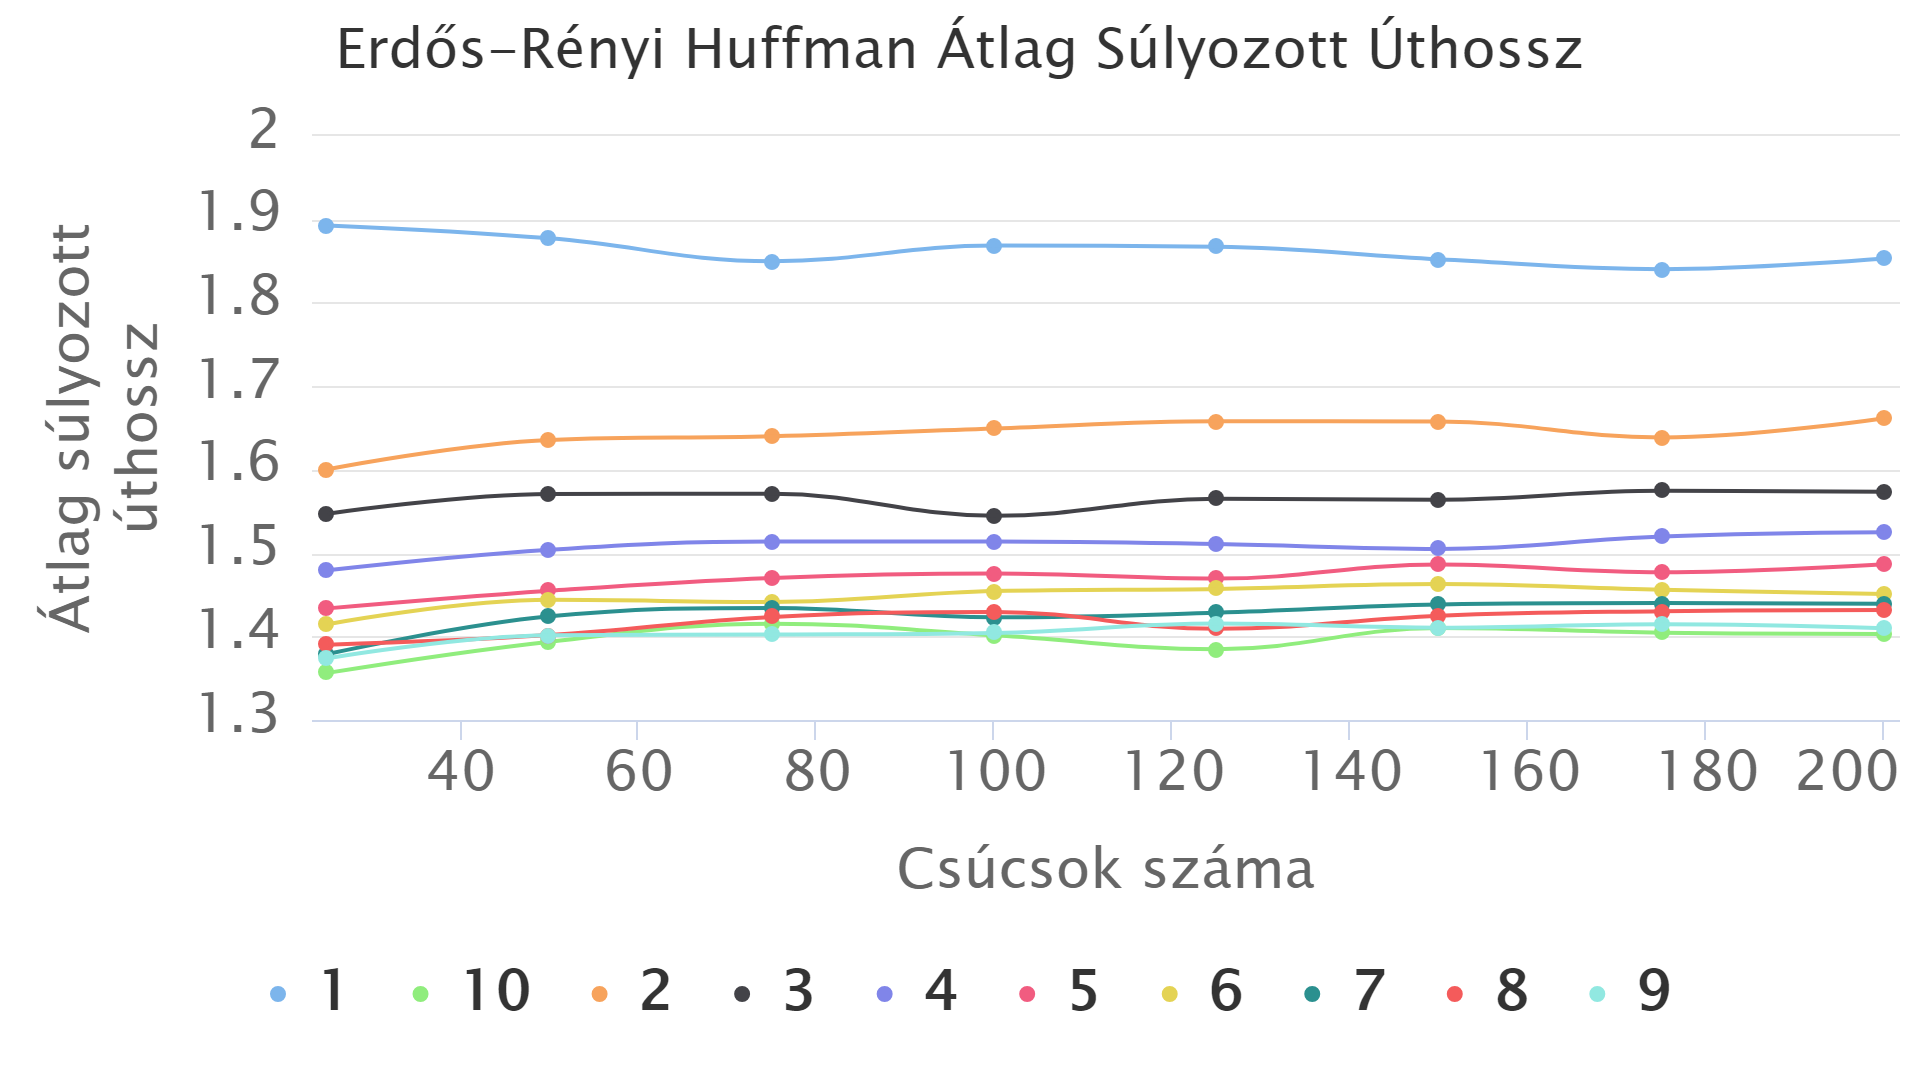
\includegraphics[width=0.49\linewidth]{pictures/erdos_avg_len_huffman.png}
		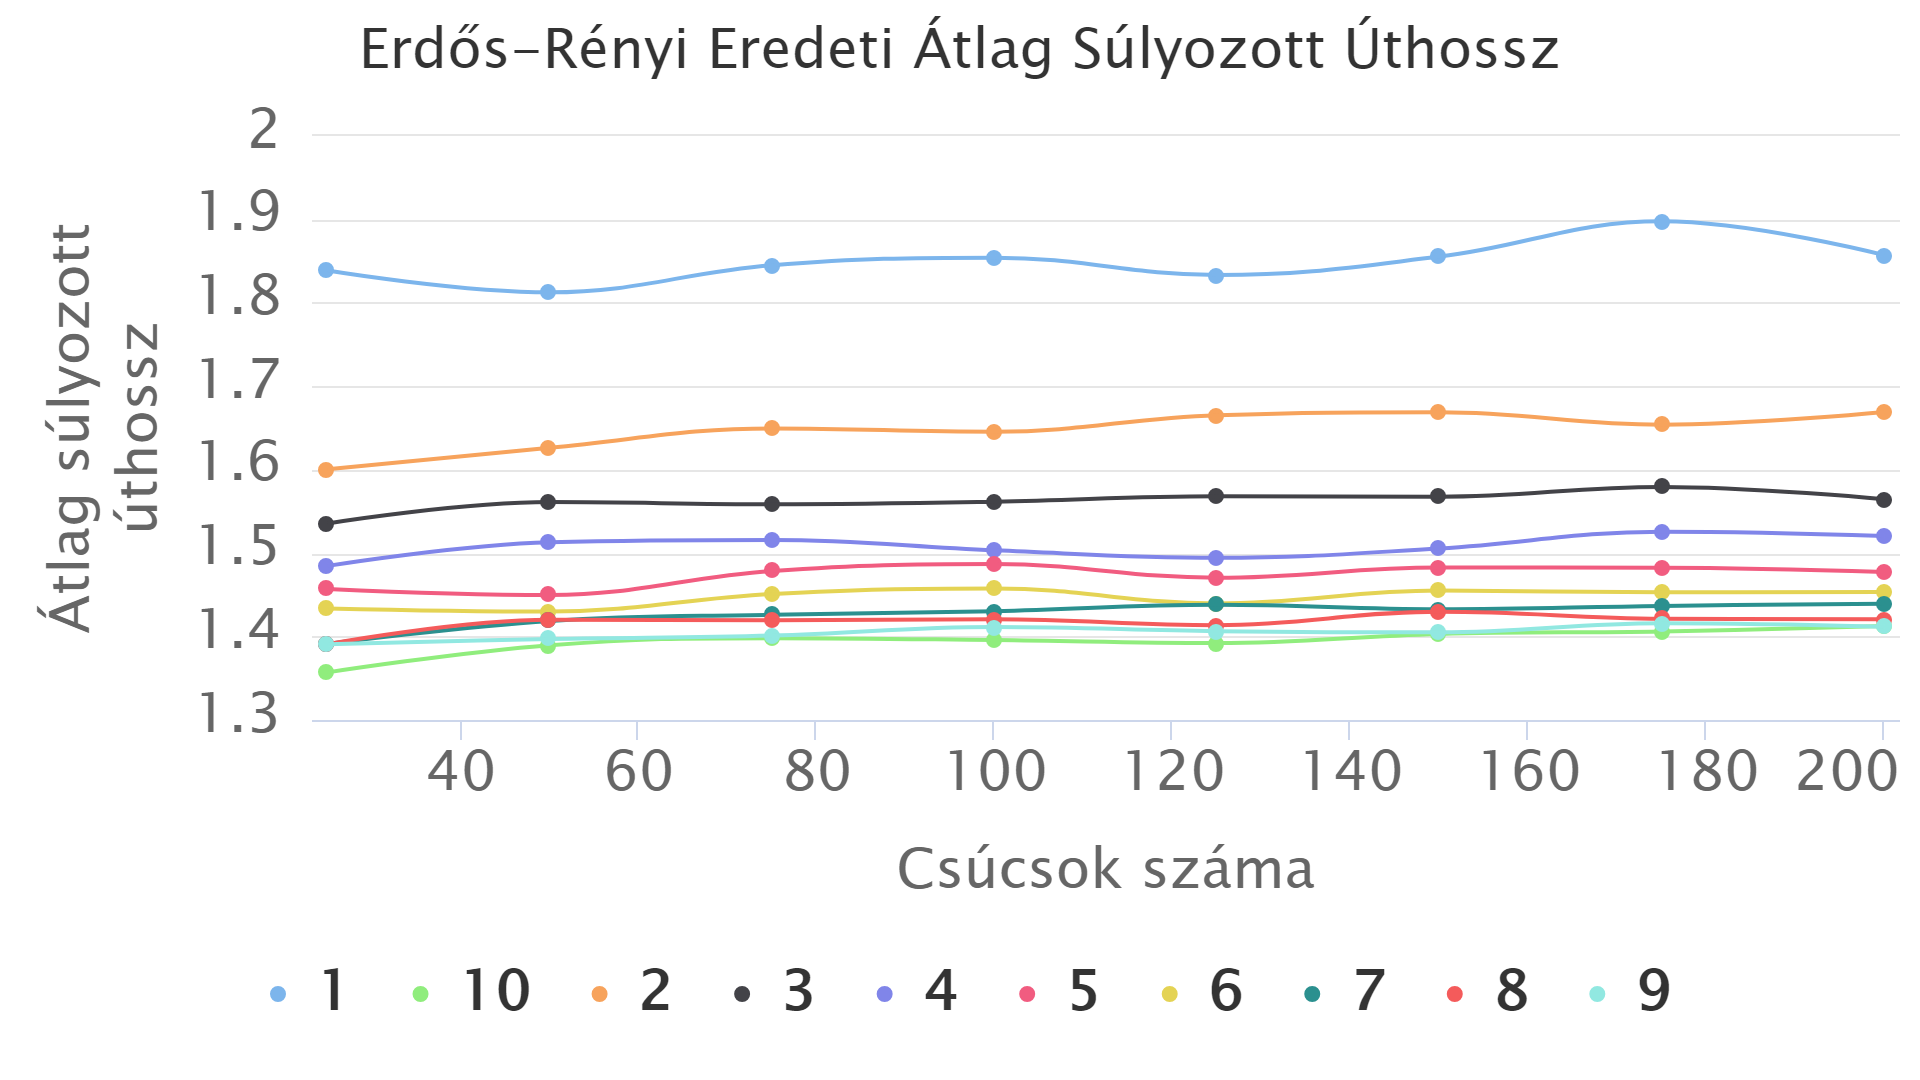
\includegraphics[width=0.49\linewidth]{pictures/erdos_avg_len_original.png}
		\caption{Átlag súlyozott úthossz Erdős-Rényi Gráf}
		\label{avg-len-erdos-renyi}
	\end{center}
\end{figure}

\subsection{Átlag torlódás}

Az átlagos úthossz eredményei már kicsit érdekesebb eredményt mutatnak.
Első megállapítás, hogy itt egyértelműen két csoportba lehet sorolni az algoritmusokat, attól függően milyen fát használták alapnak.
Az eredeti és az EgoBalance algoritmusok figyelnek a torlódás tényezőre is, ezért egyértelműen látszik a grafikonon, hogy jobban teljesítenek.
A Huffman és sorfolyonos algoritmus nem veszi számításba ezt a tényezőt, ezért nem is teljesítenek olyan jól.


\begin{figure}[h]
	\begin{center}
		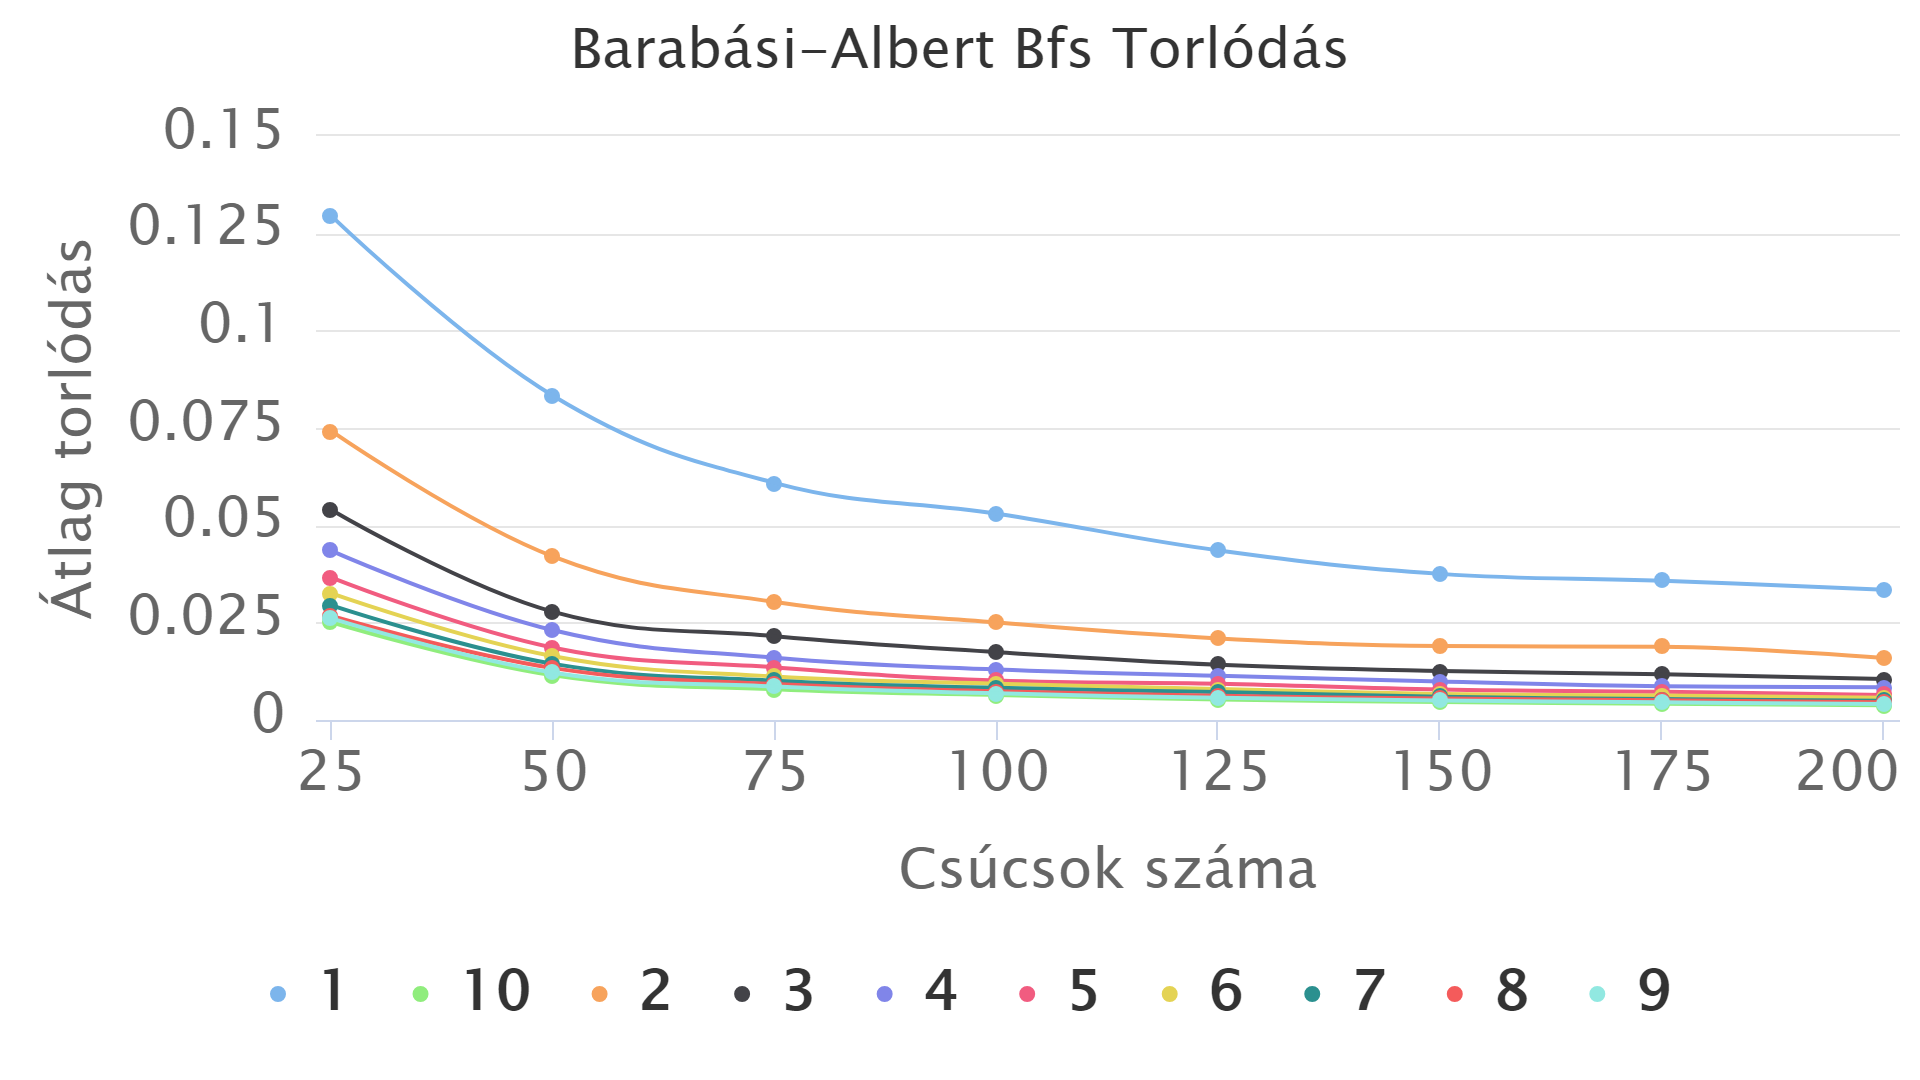
\includegraphics[width=0.49\linewidth]{pictures/barabasi_con_bfs.png}
		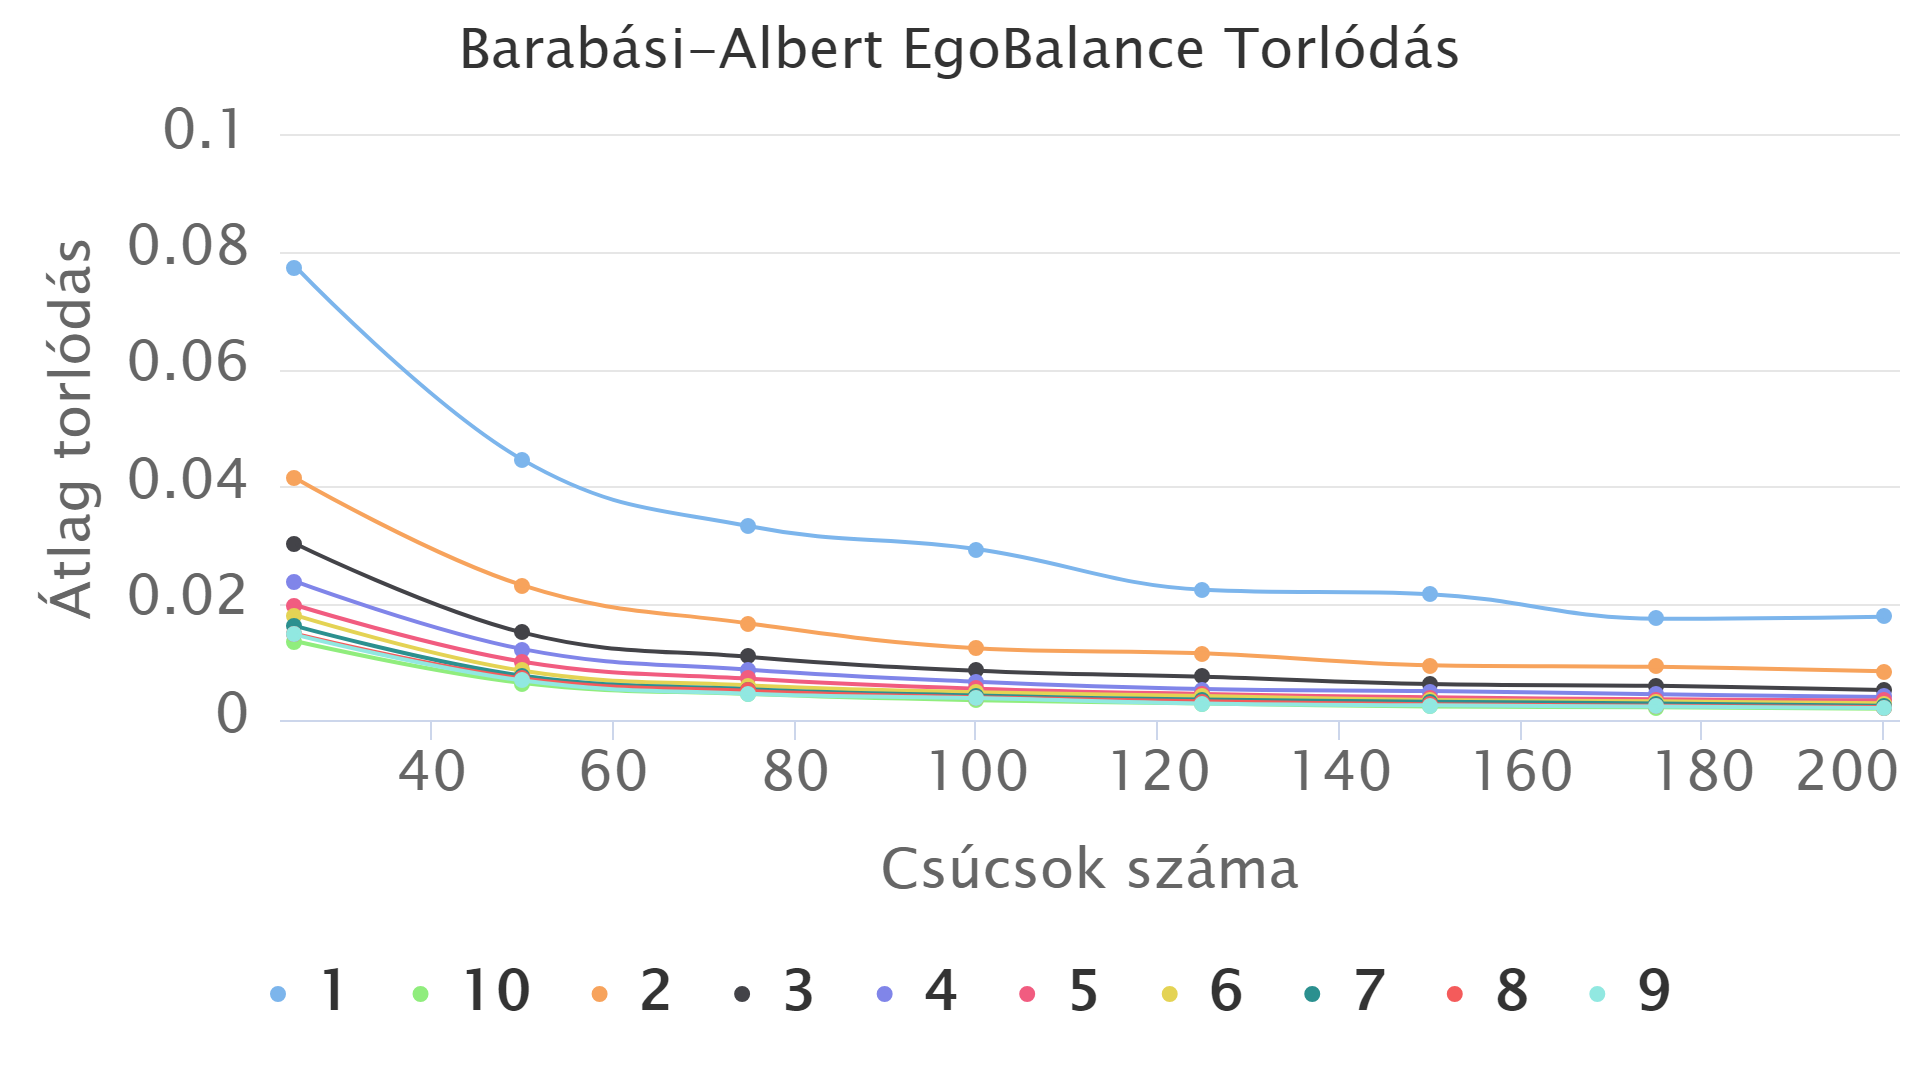
\includegraphics[width=0.49\linewidth]{pictures/barabasi_con_egobalance.png}
		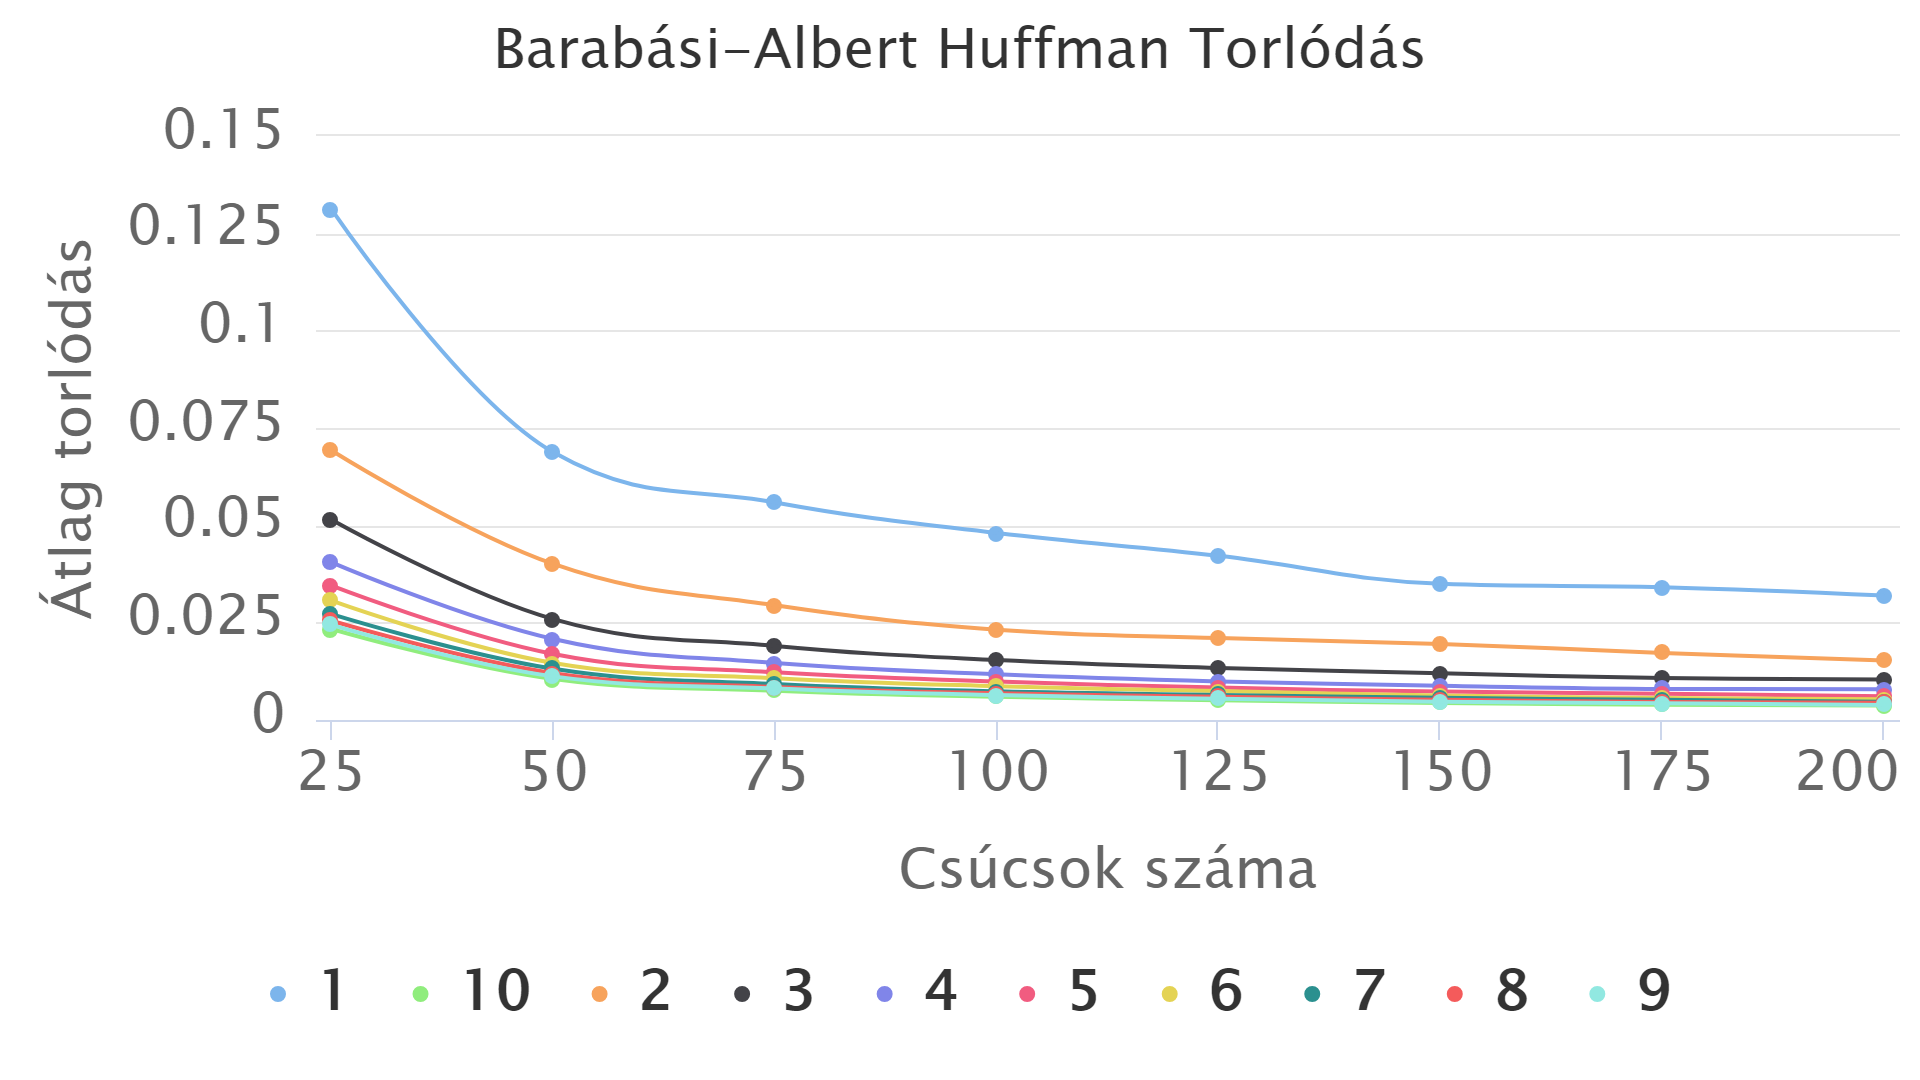
\includegraphics[width=0.49\linewidth]{pictures/barabasi_con_huffman.png}
		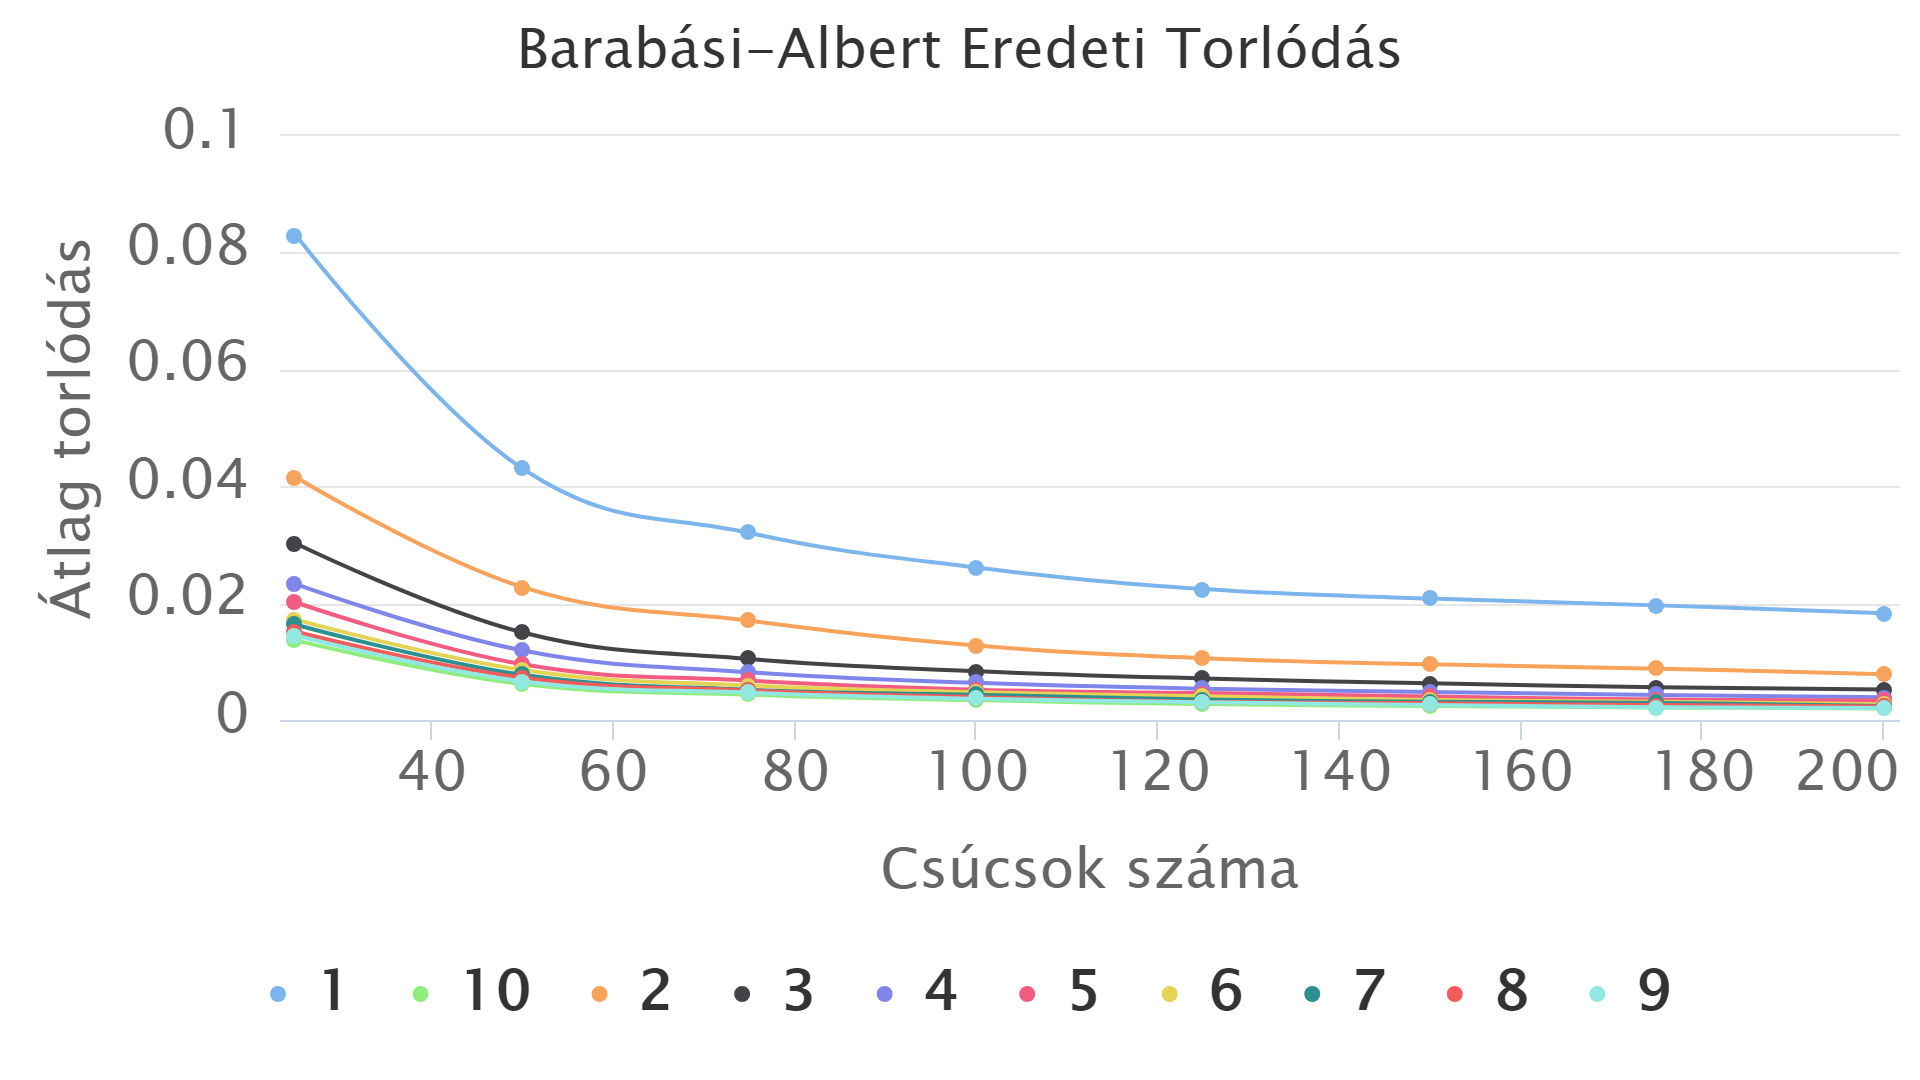
\includegraphics[width=0.49\linewidth]{pictures/barabasi_con_original.png}
		\caption{Átlag torlódás Barabási-Albert Gráf}
		\label{avg-con-barabasi}
	\end{center}
\end{figure}


\begin{figure}[h]
	\begin{center}
		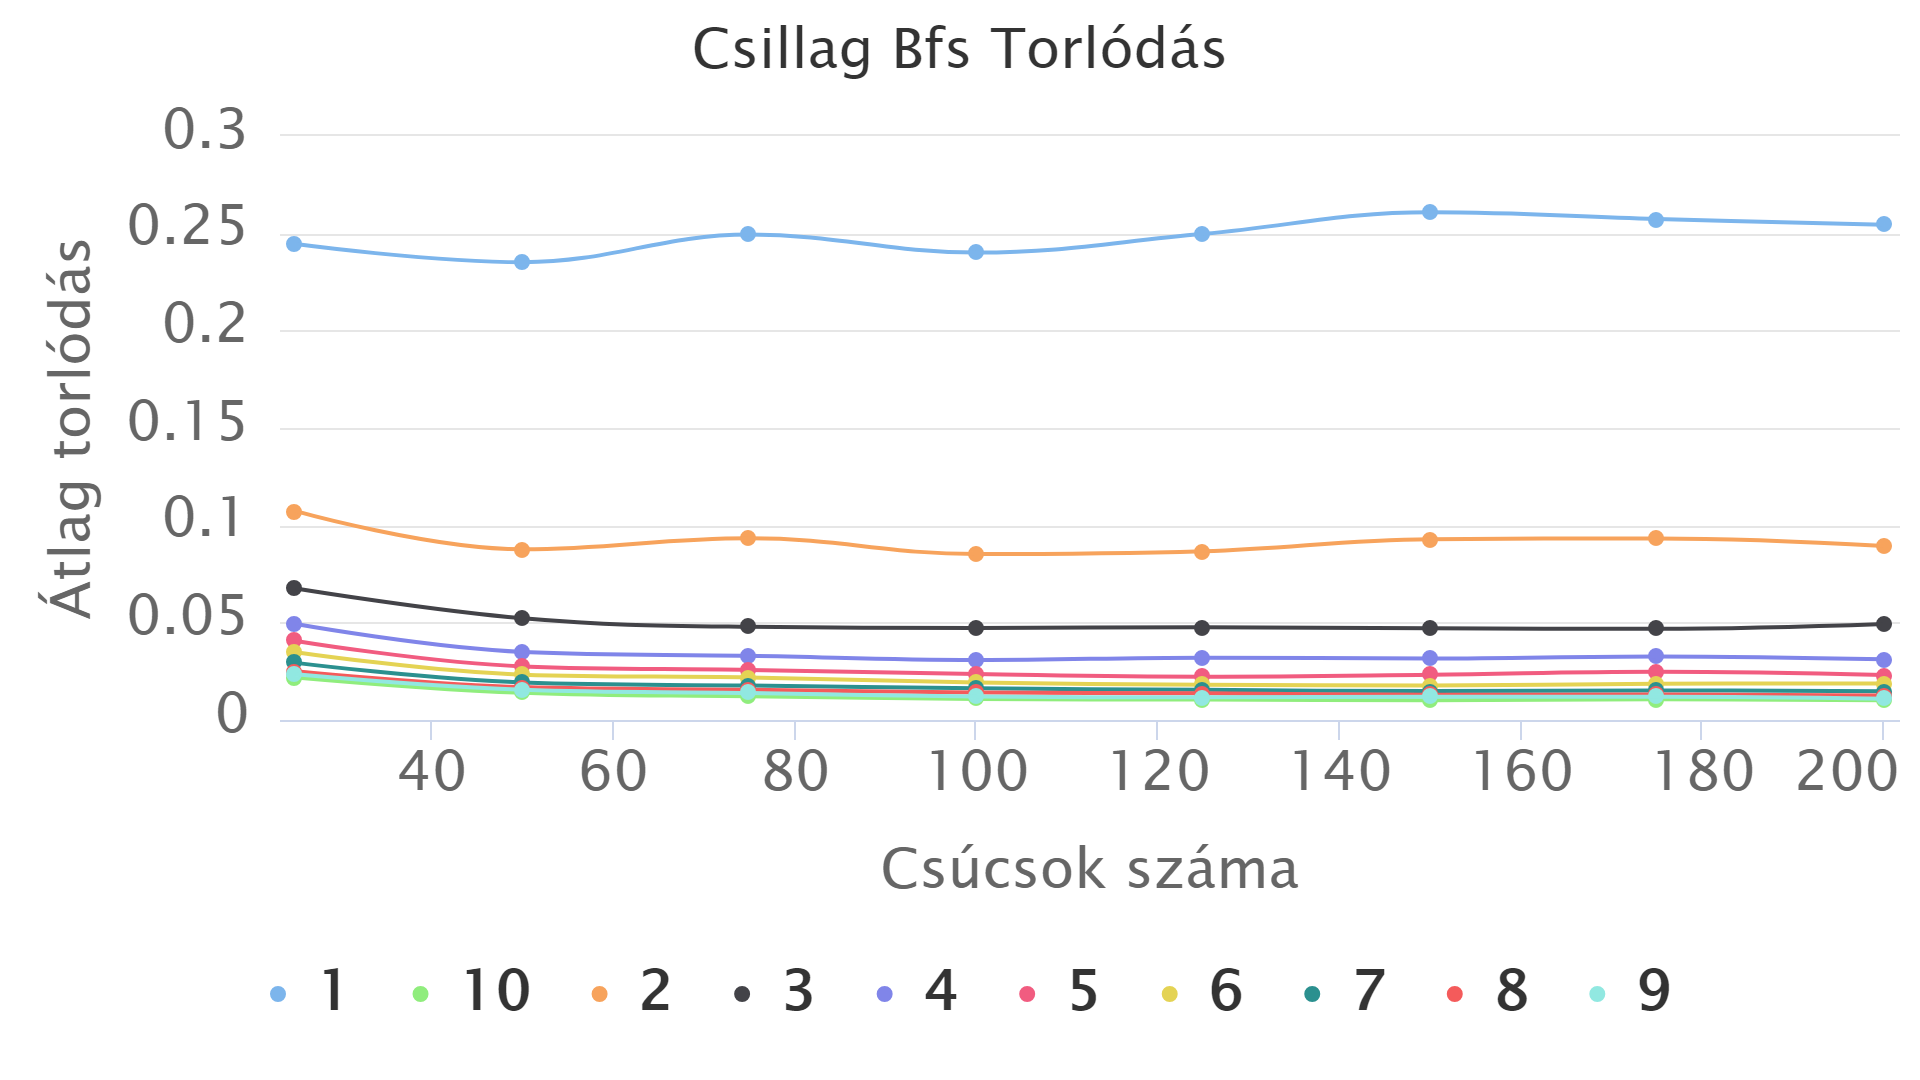
\includegraphics[width=0.49\linewidth]{pictures/star_con_bfs.png}
		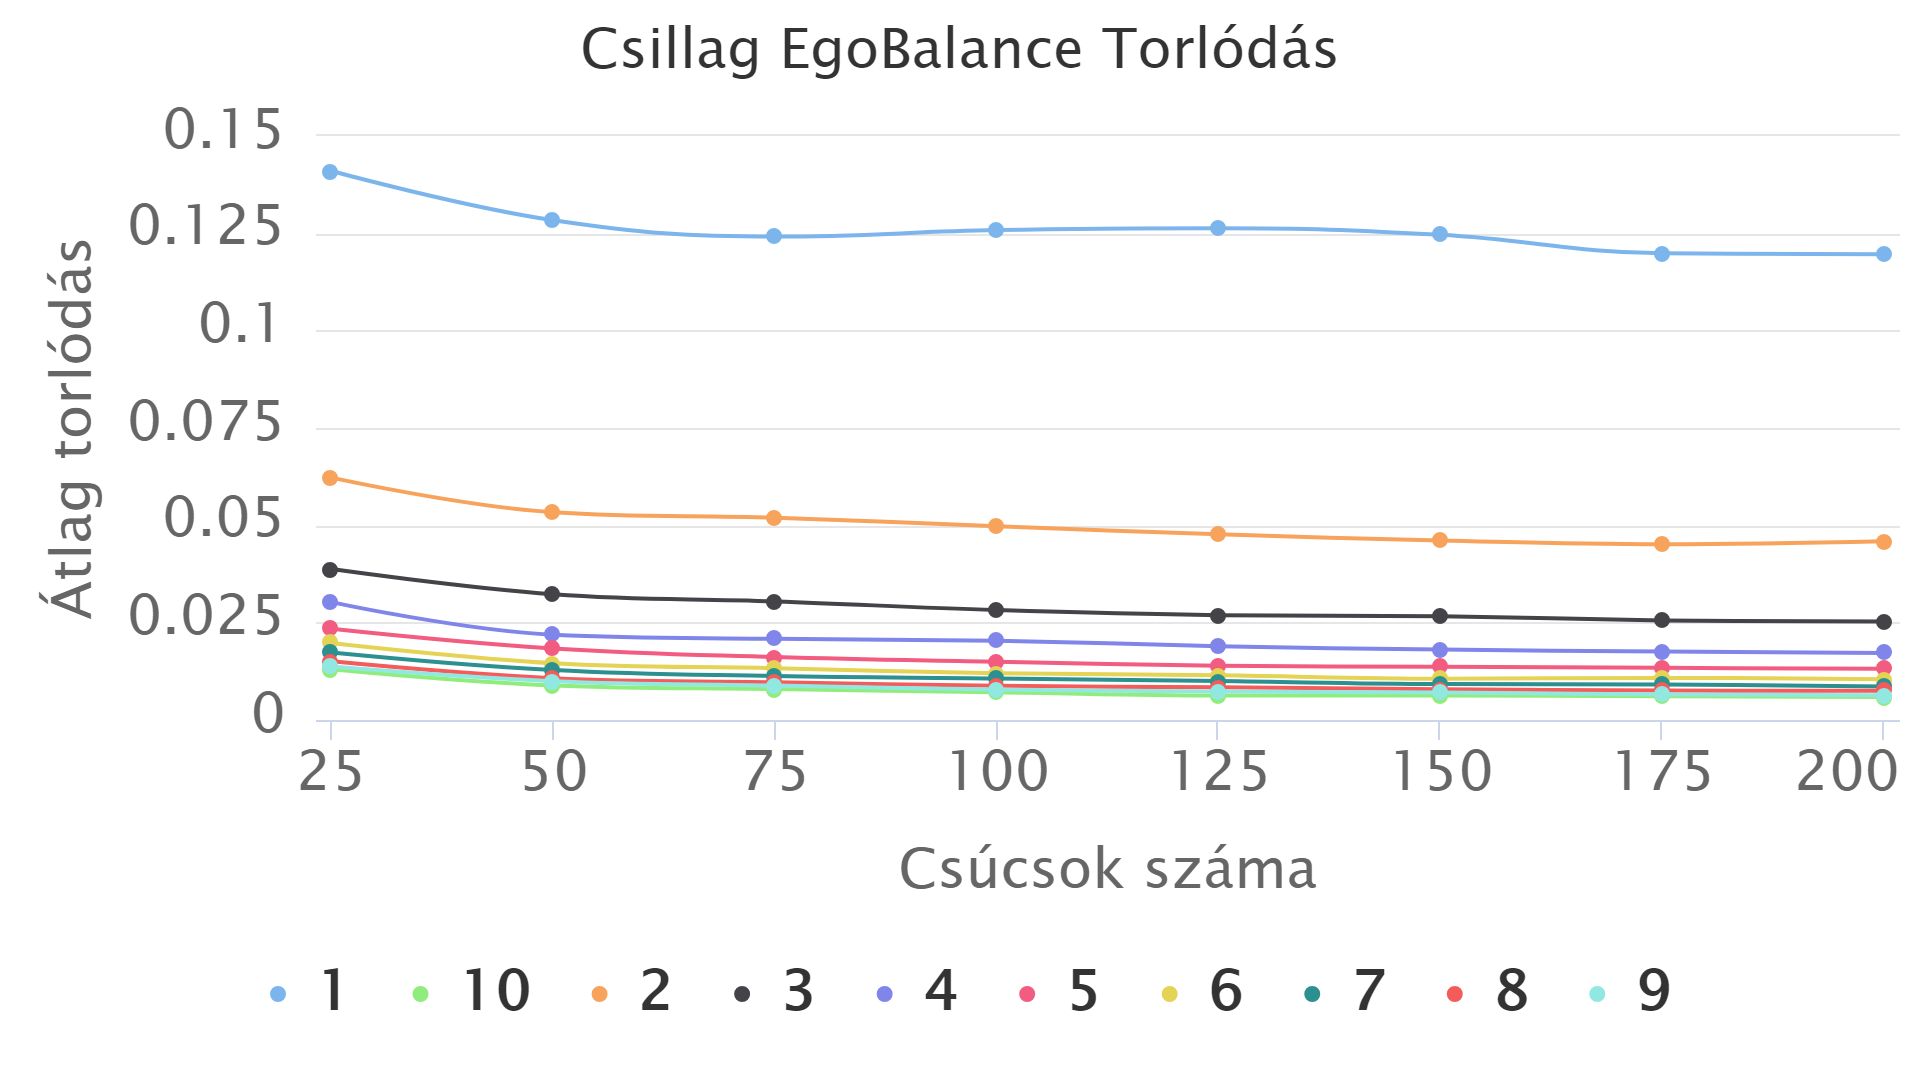
\includegraphics[width=0.49\linewidth]{pictures/star_con_egobalance.png}
		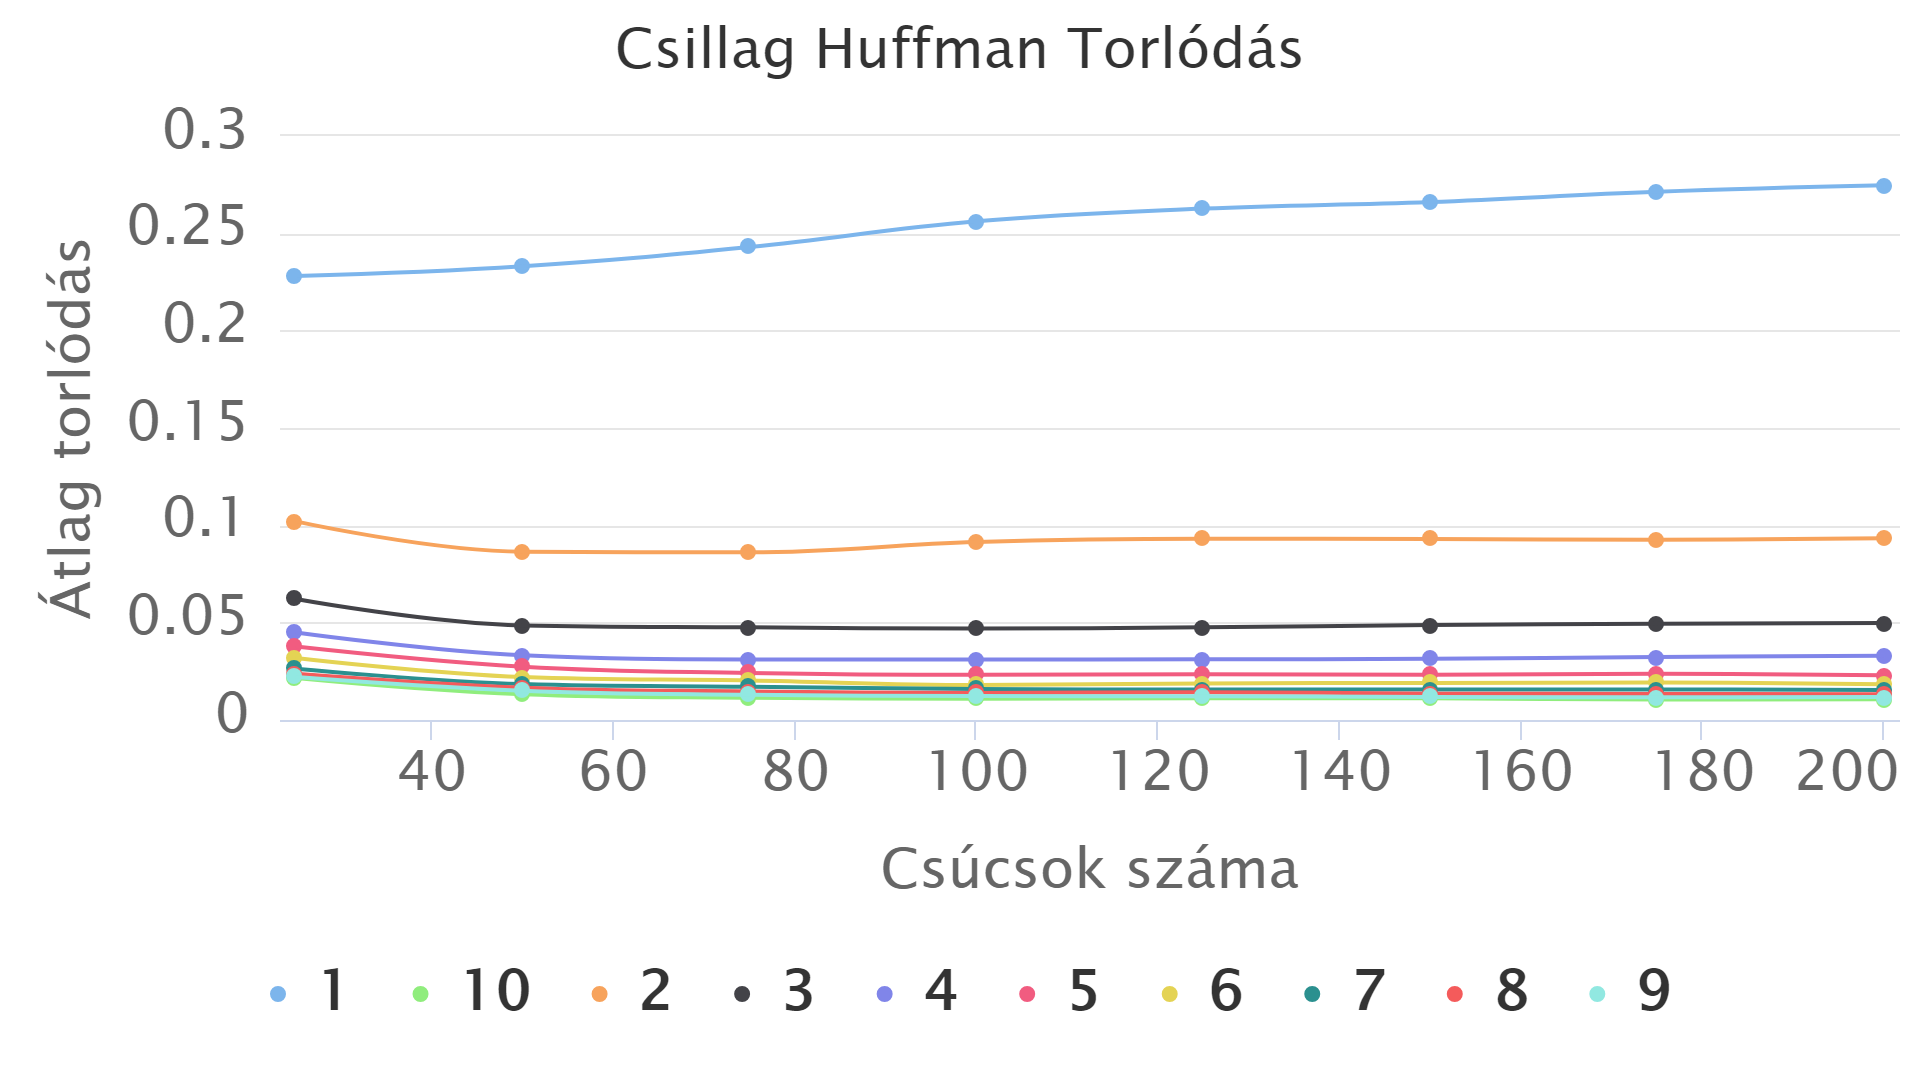
\includegraphics[width=0.49\linewidth]{pictures/star_con_huffman.png}
		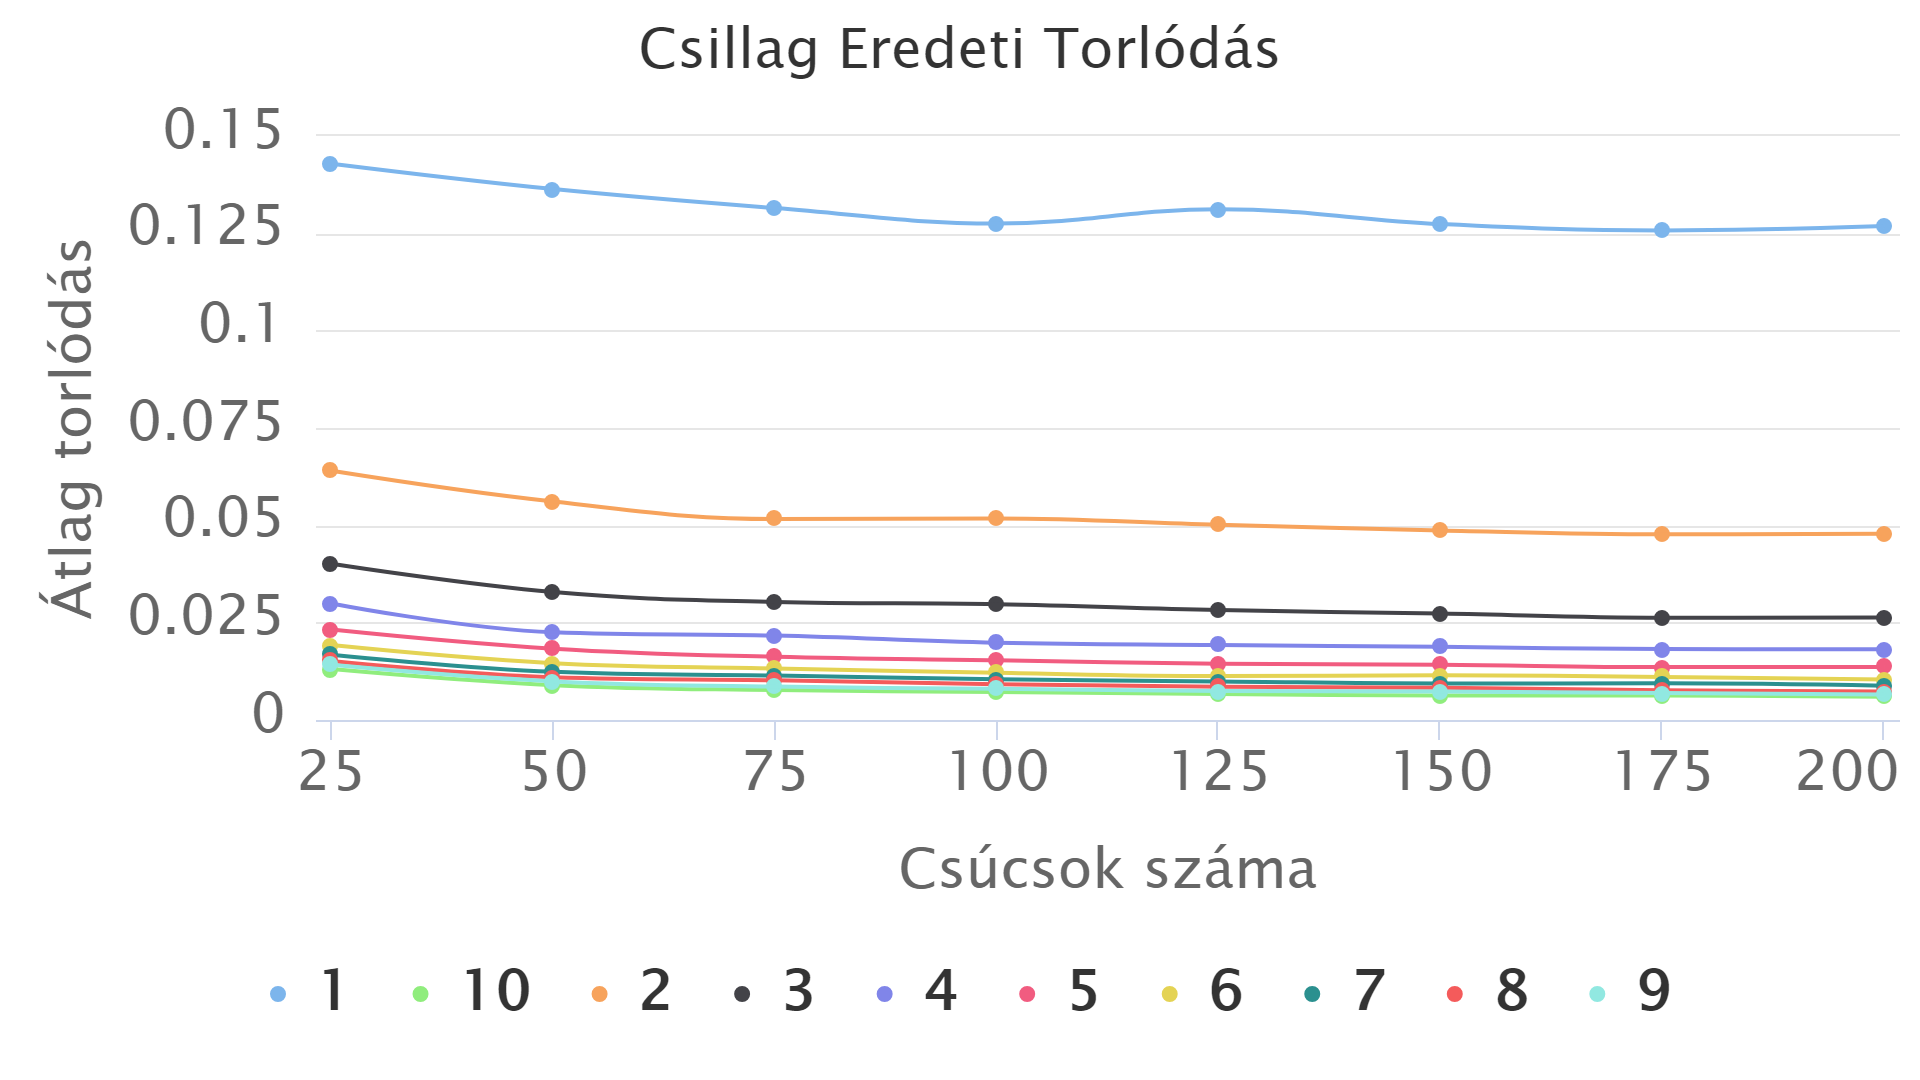
\includegraphics[width=0.49\linewidth]{pictures/star_con_original.png}
		\caption{Átlag torlódás Csillag Gráf}
		\label{avg-con-star}
	\end{center}
\end{figure}

\begin{figure}[h]
	\begin{center}
		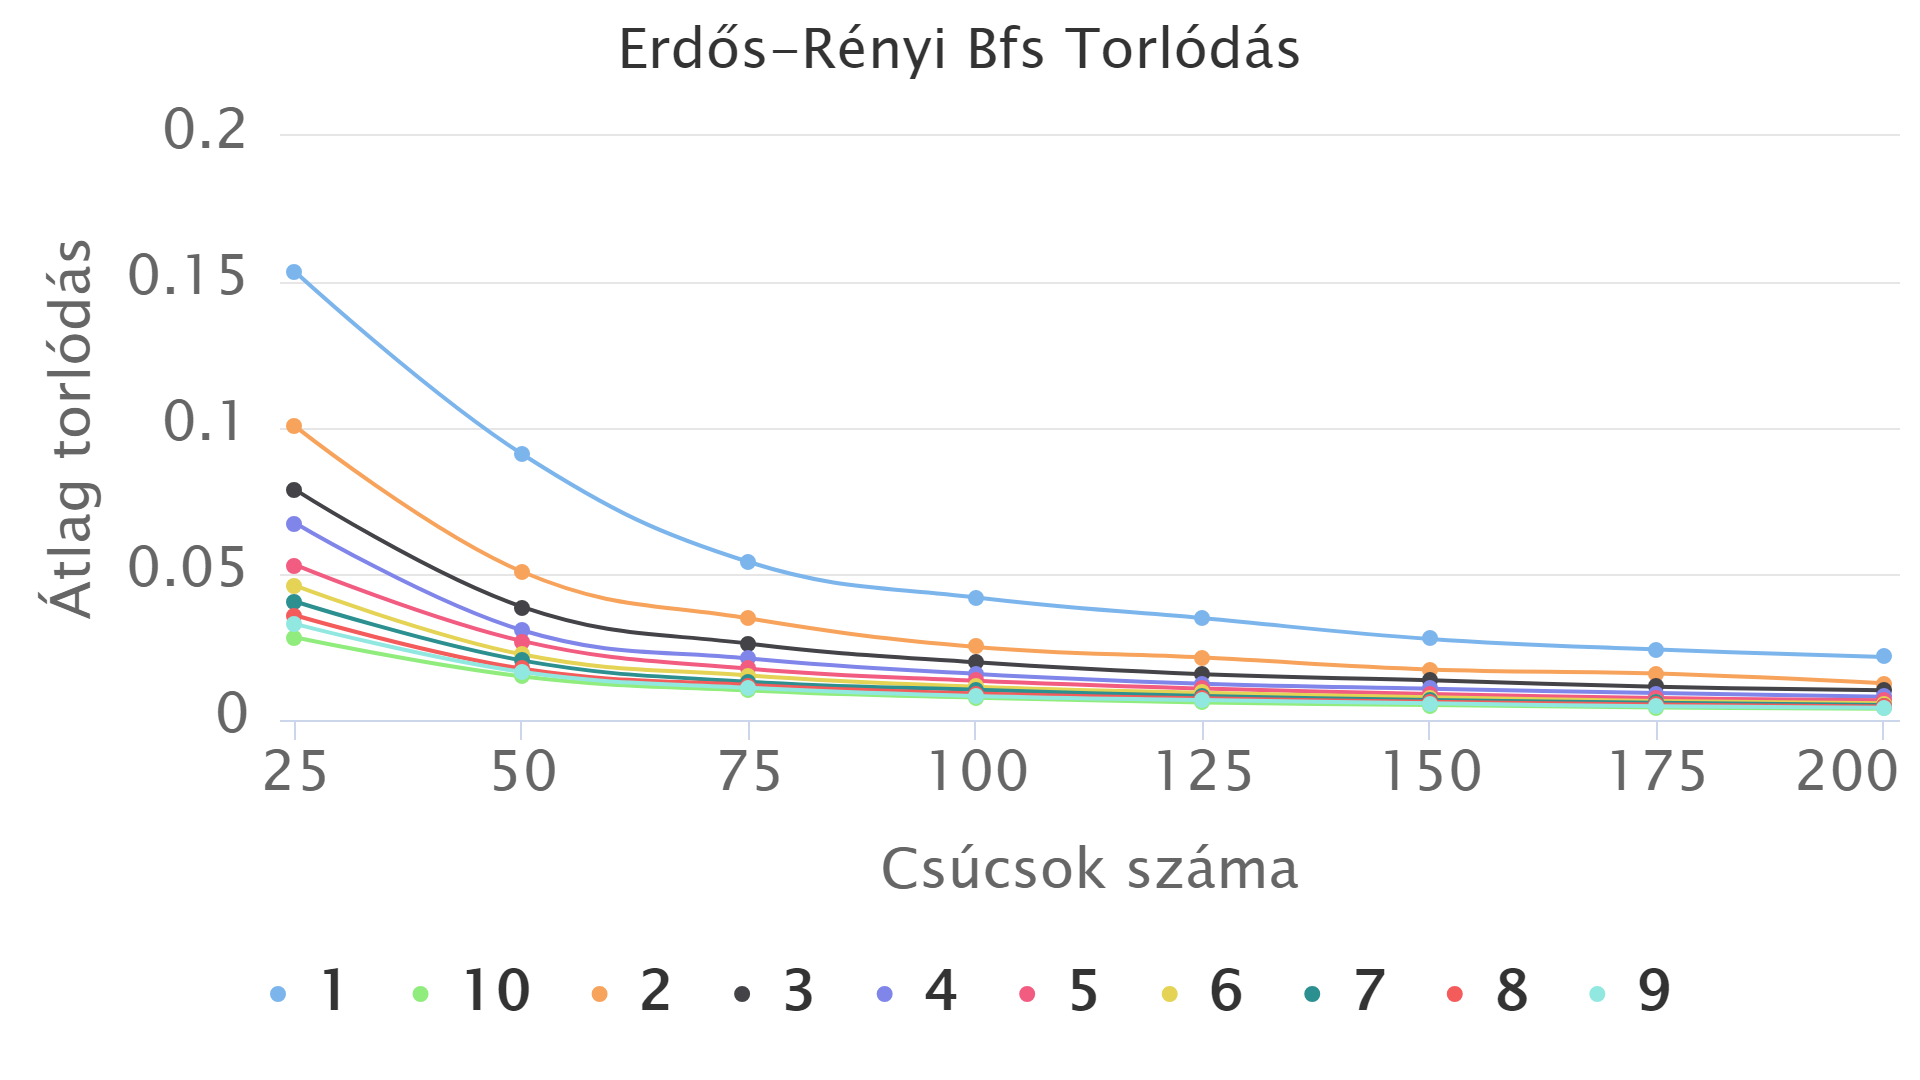
\includegraphics[width=0.49\linewidth]{pictures/erdos_con_bfs.png}
		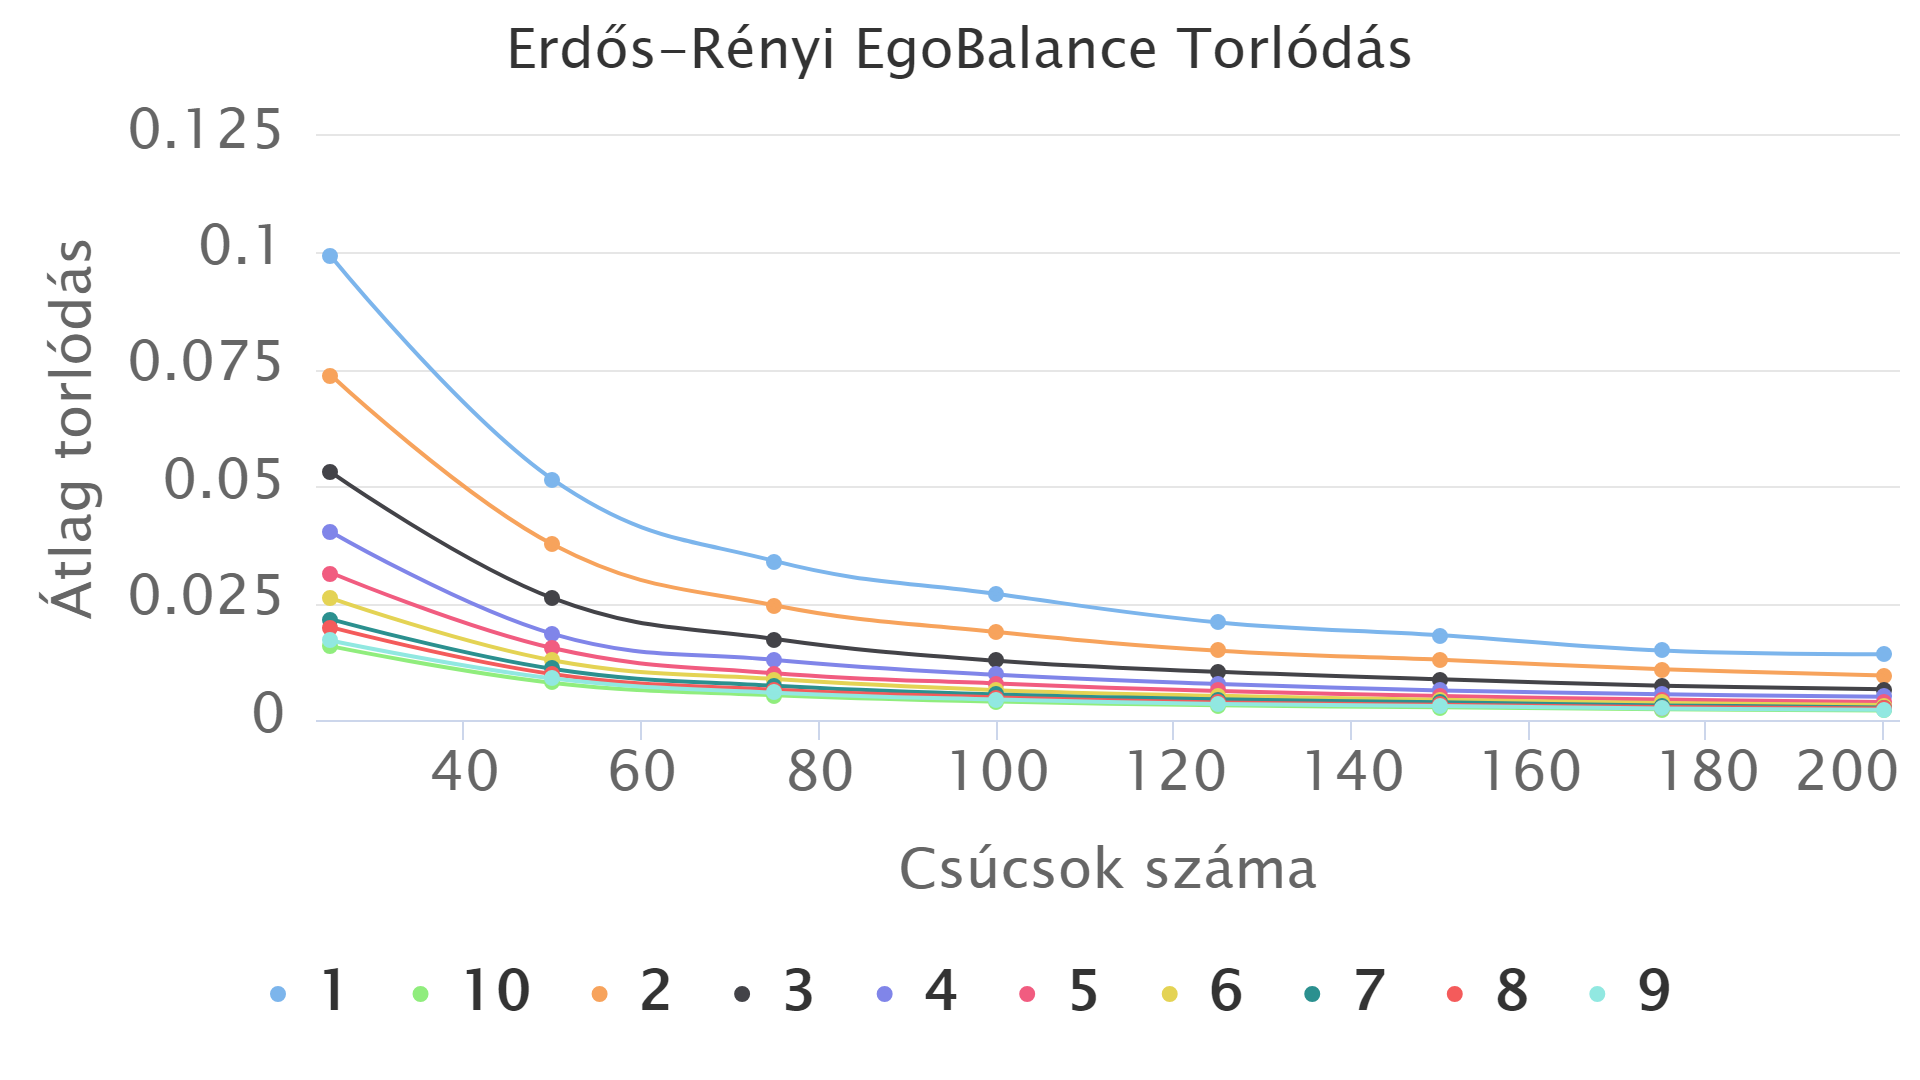
\includegraphics[width=0.49\linewidth]{pictures/erdos_con_egobalance.png}
		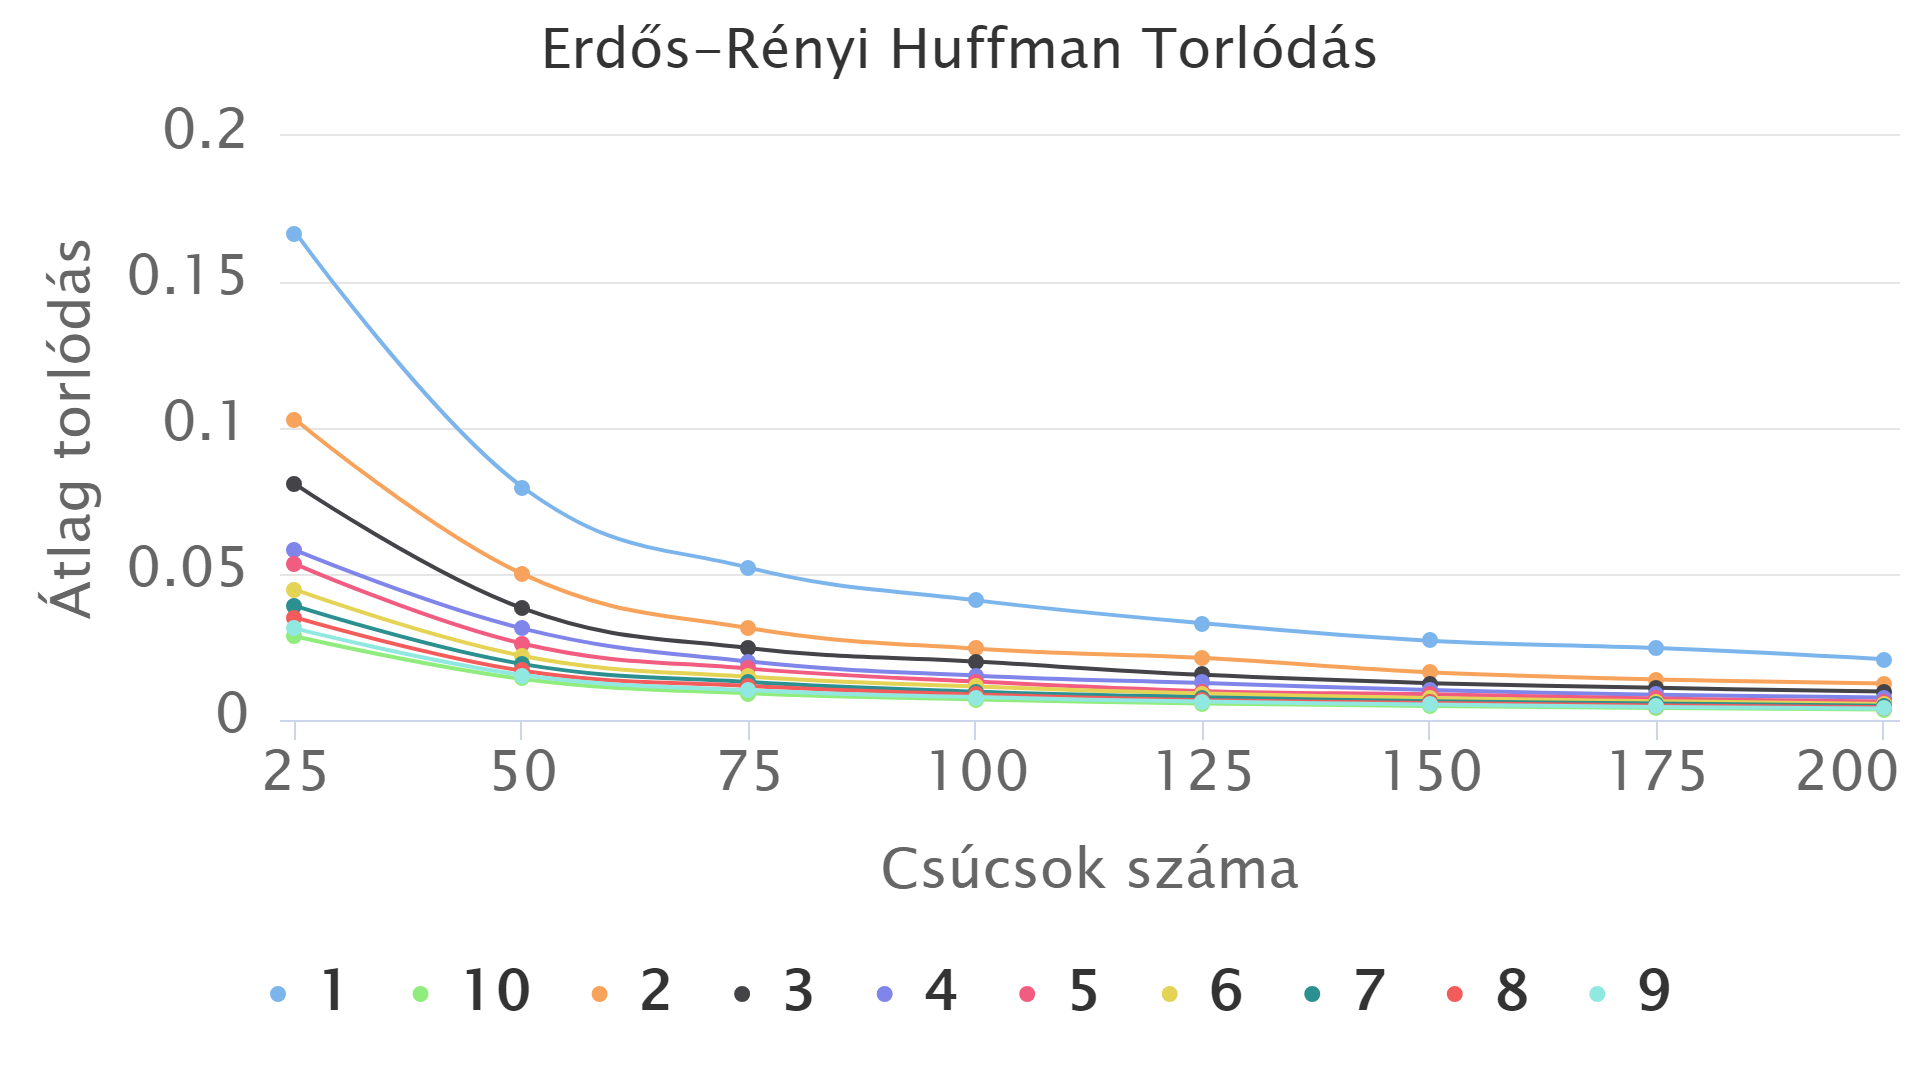
\includegraphics[width=0.49\linewidth]{pictures/erdos_con_huffman.png}
		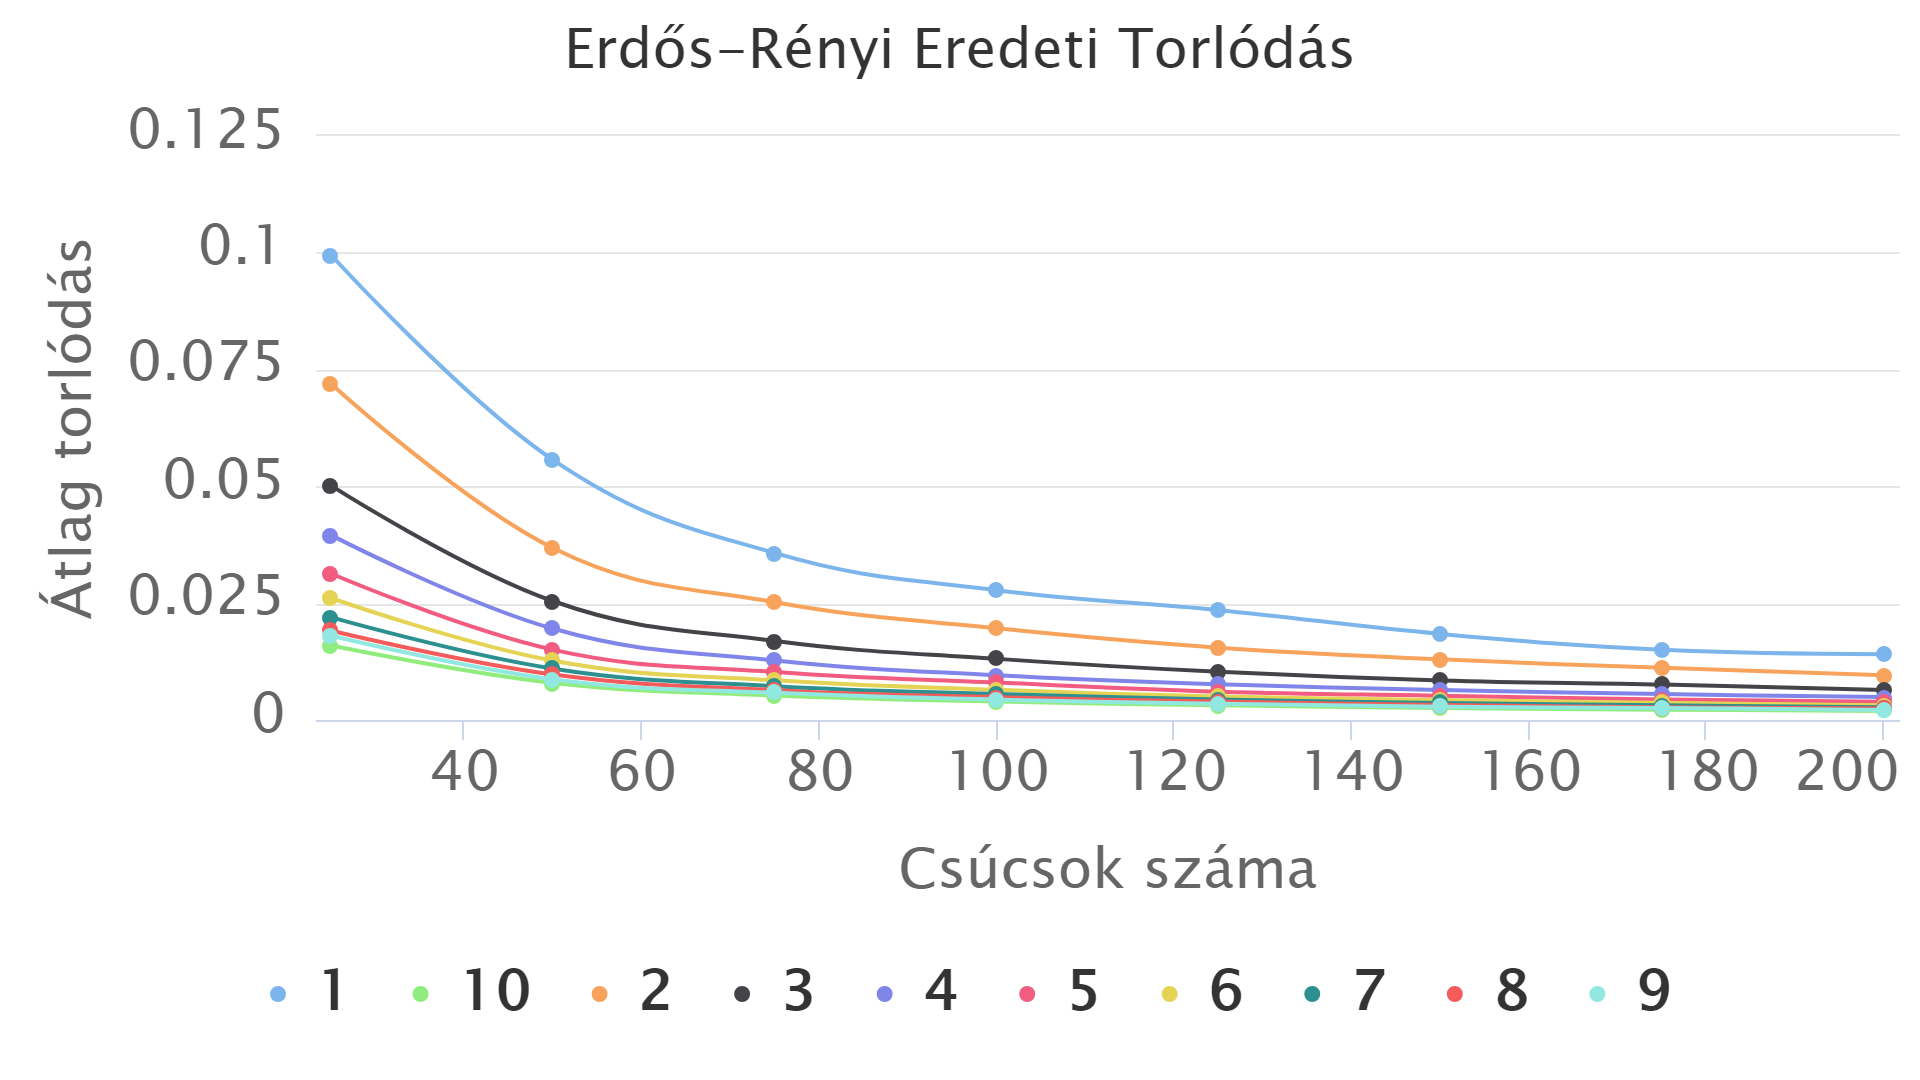
\includegraphics[width=0.49\linewidth]{pictures/erdos_con_original.png}
		\caption{Átlag torlódás Erdős-Rényi Gráf}
		\label{avg-con-erdos-renyi}
	\end{center}
\end{figure}



\chapter{Összefoglalás}

\section{Labor eredménye}

A tesztek kiértékelésének eredménye azt mutatja, hogy mind a négy algoritmus helytálló, mert hasonló eredményeket kapunk.
Az úthosszra nézve az algoritmusok teljesítménye szintén nagyon hasonló és benne van mérési hiba tartományában.
A torlódásra nézve van jelentős különbség, a Huffman fa alapú algoritmusok nem veszik figyelembe egyáltalán a torlódást, ezért határozottan rosszabbul teljesítenek.
 
Két algoritmus ami hasonló módon építi fel a fát az a sorfolytonos (Bfs) és az EgoBalance algoritmus. 
A kettő közötti lényeges különbség, amíg az Egofa legnehezebbtől legkönnyebbig próbálja a legjobban elosztani a súlyokat, addig a sorfolytonos folyamatosan rakja fel őket.
Egy ilyen kis eltérés határozottan jobb eredményhez vezet az Egofák esetén.

A végső összesítésből az látszik, hogy a szerzők által felvázolt Egofa egy megfelelő adatszerkezet arra a célra, hogy hálózatot építünk vele, ami mindkét szempontól jó eredményt eredményez.


\bibliographystyle{abbrv}
\bibliography{refrences}

	
\end{document}